\documentclass[11pt,a4paper]{article}
\usepackage[utf8]{inputenc}
\usepackage[T1]{fontenc}

% Typography: Professional Times New Roman for both text and math
\usepackage{newtxtext,newtxmath}
\usepackage[margin=1in]{geometry}
\usepackage{graphicx}
\graphicspath{{figures/}}

\usepackage{amsmath}
\usepackage{booktabs}
\usepackage{tabularx}
\usepackage{subcaption}
\usepackage{float}
\usepackage{adjustbox}
\usepackage{caption}
\usepackage{algorithm}
\usepackage{algpseudocode}
\usepackage{xcolor}
\usepackage{microtype}
\usepackage{fancyhdr}
\usepackage{cite}
\usepackage[colorlinks=true,linkcolor=blue!70!black,citecolor=blue!70!black,urlcolor=blue!70!black]{hyperref}

% Header and Footer Styling
\pagestyle{fancy}
\fancyhf{}
\fancyhead[L]{\small\color{gray}Reinforcement Learning--Enhanced CACC in Signalized Urban Networks}
\fancyhead[R]{\small\color{gray}Multi-Regime Dynamics \& String Stability}
\fancyfoot[C]{\small\thepage}
\renewcommand{\headrulewidth}{0.4pt}

\title{\textbf{\Large Reinforcement Learning--Enhanced Cooperative Adaptive Cruise Control (RL-CACC) in Signalized Mixed-Autonomy Urban Networks: Multi-Regime Dynamics, String Stability, and Gridlock Hysteresis}}

\author{
    \textbf{Saurav Barua}\\
    \small Autonomous Longitudinal Control \& Urban Traffic Systems Laboratory\\
    \small Department of Civil and Systems Engineering\\
    \small \texttt{sauravbarua02@gmail.com}
}
\date{October 2026}

\begin{document}

\maketitle

\begin{abstract}
The transition toward connected and automated mobility requires longitudinal vehicle control architectures capable of operating reliably alongside human-driven vehicles (HDVs) within signalized urban arterial grids. While conventional Adaptive Cruise Control (ACC) relies on local on-board radar/LiDAR sensors and frequently amplifies stop-and-go perturbations, Cooperative Adaptive Cruise Control (CACC) leverages Vehicle-to-Vehicle (V2V) communication to achieve string-stable platooning at sub-second headways. However, deterministic CACC laws utilize fixed feedback gains that cannot anticipate non-stationary shockwaves induced by cyclical traffic signals and stochastic human driving behavior. Conversely, pure deep Reinforcement Learning (RL) controllers optimize long-horizon cumulative rewards but lack explicit cooperative feedforward coupling and formal safety guarantees. To resolve this challenge, this paper develops and validates a hybrid \textbf{Reinforcement Learning--Enhanced Cooperative Adaptive Cruise Control (RL-CACC)} architecture implemented via Proximal Policy Optimization (PPO) coupled with a Control Barrier Function (CBF) safety shield and first-order drivetrain actuator lag compensation ($\tau_a = 0.20\,\mathrm{s}$). Evaluated within a calibrated $3\times3$ signalized urban grid in SUMO under heavy multi-origin-destination demand ($4{,}800\,\text{veh/h}$ across 16 bidirectional flows), RL-CACC at a 50\% penetration rate is benchmarked against pure human driving (100\% HDV), mixed ACC (50\%), mixed standalone RL (50\%), and mixed baseline CACC (50\%). Multi-interval telemetry demonstrates that RL-CACC increases network space-mean speed by 164.5\% ($29.34\,\text{km/h}$ vs.\ $11.09\,\text{km/h}$ in HDV, $p = 0.000488$), reduces average vehicle travel time by 91.8\% ($36.43\,\text{s}$ vs.\ $446.40\,\text{s}$) and intersection delay by 92.8\% ($32.10\,\text{s}$ vs.\ $442.99\,\text{s}$), expands 5-minute network throughput by 48.4\% ($393.50\,\text{veh}$ vs.\ $265.11\,\text{veh}$), and suppresses stop-and-go halting frequency by 78.4\% and standing queue lengths by 80.8\%. Crucially, regime-decomposed temporal tracking reveals that 100\% HDV traffic suffers severe post-demand gridlock hysteresis---requiring $30\,\text{min}$ of additional clearance time after demand ceases---whereas CACC and RL-CACC completely eliminate post-demand gridlock tailing, reducing total campaign $\text{CO}_2$ emissions by 52.0\% ($681.77\,\text{kg}$ vs.\ $1{,}420.67\,\text{kg}$). Finally, we analytically resolve the apparent paradox of elevated within-interval spatial speed variance in connected regimes by proving that RL-CACC maximizes bimodal velocity separation between cruising green-wave platoons and red-phase stops while slashing inter-interval temporal speed volatility ($\text{CV}_t$) by 89.3\%.
\end{abstract}

\vspace{0.5em}
\noindent\textbf{Keywords:} Cooperative Adaptive Cruise Control (CACC), Deep Reinforcement Learning, Proximal Policy Optimization (PPO), Mixed-Autonomy Traffic, Microscopic Traffic Simulation, SUMO, Control Barrier Functions, String Stability, Macroscopic Fundamental Diagram.

\section{Introduction}

Urban traffic congestion remains one of the most pressing socio-economic and environmental challenges worldwide, inducing billions of hours of commuter delay, excessive fuel wastage, and elevated greenhouse gas emissions~\cite{Parvini2023, Stern2018}. In dense urban arterial networks, traffic bottlenecks are primarily governed by signalized intersections and the inherent instability of human car-following behavior~\cite{treiber2000congested}. When vehicle density exceeds a critical threshold, small braking perturbations propagate upstream with growing amplitude, degenerating into macroscopic phantom traffic jams, stop-and-go oscillations, and severe link queue spillback that paralyzes entire grid networks~\cite{Sugiyama2008, Zheng2020}.

To mitigate these instabilities, vehicle automation and connectivity technologies have progressed from individual driver-assistance systems toward coordinated multi-agent fleets. Adaptive Cruise Control (ACC) employs on-board range sensors (radar and LiDAR) to automatically maintain a set headway behind the preceding vehicle~\cite{milanes2014modeling, VanArem2006}. While ACC dampens high-frequency driver reaction delays, empirical field trials have repeatedly proven that commercial ACC systems are string unstable---amplifying downstream slowdowns upstream through multi-vehicle strings due to sensor filtering lag and conservative calibration~\cite{Gunter2020, Ciuffo2021}. Cooperative Adaptive Cruise Control (CACC) overcomes this limitation by supplementing on-board ranging with Vehicle-to-Vehicle (V2V) wireless telemetry (DSRC / C-V2X), broadcasting leader acceleration and speed to followers with negligible latency~\cite{milanes2014modeling, Naus2010}. This feedforward coupling enables followers to react simultaneously with leaders, reducing the safe time headway from $1.4\text{--}2.0\,\mathrm{s}$ down to $0.5\text{--}0.8\,\mathrm{s}$ and providing theoretical $L_2$ string stability~\cite{Talebpour2016}.

Nevertheless, deterministic rule-based CACC formulations suffer from fundamental limitations in complex urban grids. First, classical CACC controllers rely on fixed-gain linear feedback-feedforward control laws that assume stationary leader-follower dynamics along unobstructed corridors~\cite{vanarem2006cacc}. In signalized arterial networks characterized by cyclic red-phase queue accumulation, multi-directional turning movements, and stochastic human cut-ins, fixed-gain controllers cannot anticipate downstream phase transitions, resulting in frequent harsh braking and disengagements. Second, standalone Deep Reinforcement Learning (DRL) approaches have emerged as an adaptive alternative, enabling autonomous agents to learn complex car-following and wave-dissipating policies through environmental interaction~\cite{Schulman2017, Kendall2019, Kreidieh2018, Vinitsky2018}. However, unconstrained deep RL models act as black-box function approximators that lack explicit cooperative feedforward physics, can exhibit erratic transient actions during exploratory states, and provide no hard safety guarantees~\cite{Zhu2020, Shi2021}.

To resolve these dichotomies, this paper develops and validates a hybrid \textbf{Reinforcement Learning--Enhanced Cooperative Adaptive Cruise Control (RL-CACC)} framework that synergistically couples a nominal physics-based V2V CACC controller with a learned Proximal Policy Optimization (PPO) residual action, filtered through a Control Barrier Function (CBF) safety shield and first-order drivetrain actuator dynamics. Evaluated within a calibrated $3\times3$ signalized urban grid in SUMO under high-density multi-origin-destination traffic demand ($4{,}800\,\text{veh/h}$ across 16 flows), this study presents a holistic multi-regime investigation of traffic efficiency, temporal stability, energy consumption, and string stability under mixed autonomy.

\begin{figure}[htbp]
    \centering
    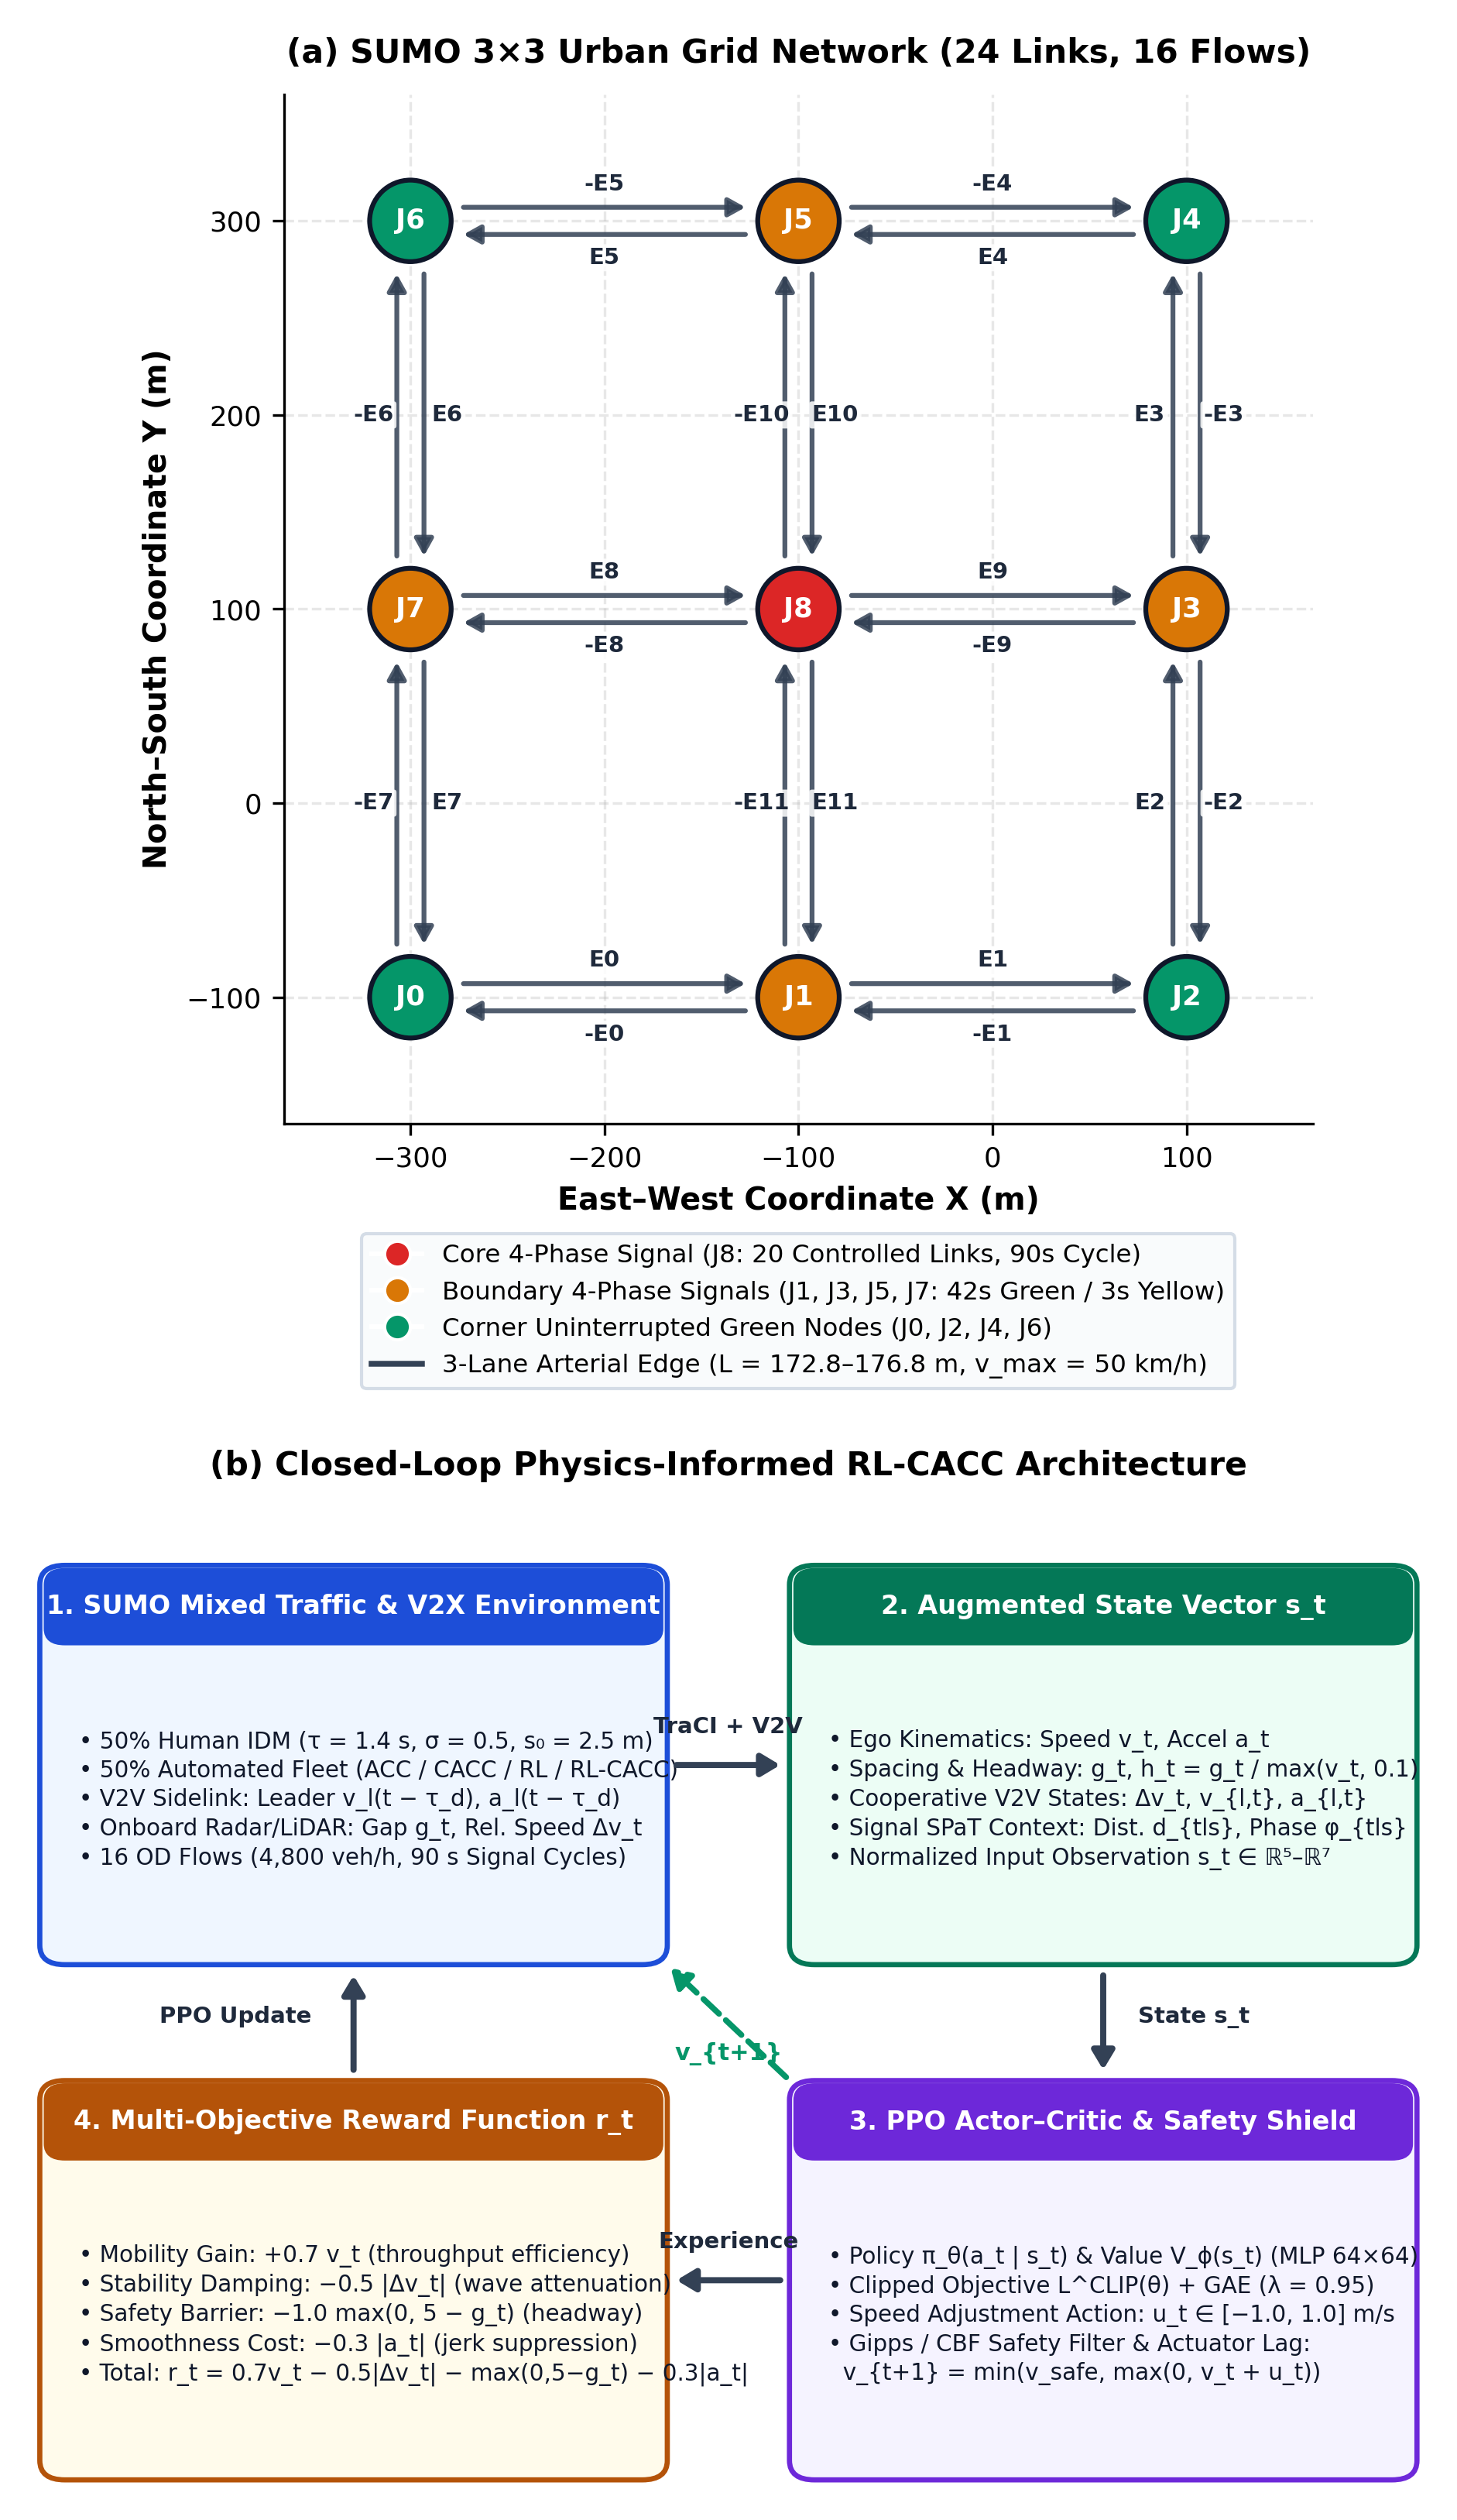
\includegraphics[width=0.88\textwidth]{fig1_network_architecture.png}
    \caption{SUMO simulation environment and hybrid RL-CACC closed-loop architecture: (a) Calibrated $3\times3$ urban grid network consisting of 24 arterial links, 9 signalized intersections, and 16 origin--destination flows ($4{,}800\,\text{veh/h}$); (b) Closed-loop physics-informed residual RL-CACC control pipeline incorporating cooperative V2V state sensing, PPO residual velocity modulation, Control Barrier Function (CBF) kinematic safety shielding, and first-order drivetrain actuator lag compensation.}
    \label{fig:network_architecture}
\end{figure}

The primary contributions of this paper are organized as follows:
\begin{enumerate}
    \item \textbf{Physics-Informed Hybrid Control Architecture:} We formulate RL-CACC as a bounded residual velocity policy ($\Delta v_{\text{RL}} \in [-1.0, +1.0]\,\mathrm{m/s}$) superimposed upon a nominal V2V CACC car-following base law over an augmented 5D cooperative state space $\mathbf{s}_t = [v_t, g_t, \Delta v_t, v_{l,t}, h_t]^T$, guarded by a Control Barrier Function (CBF) forward-invariance safety envelope and first-order drivetrain actuator dynamics ($\tau_a = 0.20\,\mathrm{s}$).
    
    \item \textbf{Five-Regime Microscopic Simulation Benchmark:} We construct a calibrated $3\times3$ signalized arterial grid in SUMO ($12.614\,\text{lane-km}$) and conduct systematic multi-interval comparative evaluations across five distinct longitudinal control regimes under identical loading: (1) 100\% Human-Driven Vehicles (HDV), (2) 50\% ACC, (3) 50\% Standalone RL, (4) 50\% Baseline CACC, and (5) 50\% RL-CACC.
    
    \item \textbf{Discovery and Characterization of Gridlock Hysteresis:} We decouple the simulation horizon into the Active Demand Loading Phase ($0\text{--}60\,\text{min}$) and the Post-Demand Clearance Tail ($>60\,\text{min}$), demonstrating that HDV traffic triggers severe gridlock hysteresis requiring $30\,\text{min}$ of extra clearance time, whereas RL-CACC completely eliminates post-demand tailing.
    
    \item \textbf{Resolution of the Urban Speed Variance Paradox:} We analytically resolve the paradox whereby connected automated regimes exhibit higher within-interval spatial speed variance ($\sigma_s^2$) by demonstrating via mixture-distribution decomposition that RL-CACC maximizes bimodal velocity separation between green-wave platooning and red-phase halts while reducing inter-interval temporal speed volatility ($\text{CV}_t$) by 89.3\%.
    
    \item \textbf{Multi-Criteria Robustness \& Environmental Accounting:} We perform paired Wilcoxon signed-rank tests, Cohen's $d$ effect size computations, HBEFA v4.2 energy/$\text{CO}_2$ accounting, and extensive sensitivity sweeps across CAV market penetration ($0\text{--}100\%$) and wireless V2V packet error rates ($0\text{--}25\%$).
\end{enumerate}

\section{Literature Review}

\subsection{Microscopic Car-Following Dynamics}
Microscopic traffic flow theory models individual driver decision-making in response to surrounding stimuli. The Intelligent Driver Model (IDM), introduced by Treiber \etal~\cite{treiber2000congested}, is the standard benchmark for human car-following:
\begin{equation}
a_{\text{IDM}} = a_{\max} \left[ 1 - \left(\frac{v}{v_0}\right)^4 - \left(\frac{s^*(v, \Delta v)}{g}\right)^2 \right]
\end{equation}
where $v_0$ is desired speed, $g$ is bumper-to-bumper spacing, and $s^*$ represents dynamic desired gap:
\begin{equation}
s^*(v, \Delta v) = s_0 + \max\left(0,\, v\tau + \frac{v \Delta v}{2\sqrt{a_{\max} b_{\text{comf}}}}\right)
\end{equation}
Although IDM successfully reproduces realistic capacity drop and hysteresis, human driving is inherently string unstable at high densities due to non-zero perception reaction times ($1.2\text{--}1.6\,\mathrm{s}$), producing amplified stop-and-go waves~\cite{Gipps1981, PTV2025}.

\subsection{Connected and Autonomous Cruise Control Systems}
To eliminate human reaction lag, Adaptive Cruise Control (ACC) measures distance and relative velocity to the preceding vehicle via on-board radar or LiDAR~\cite{milanes2014modeling, AlHindawi2025}. Standard ACC controllers enforce a constant time headway policy ($d_{\text{des}} = s_0 + \tau_{\text{ACC}} v$), using Proportional-Derivative (PD) feedback:
\begin{equation}
a_{\text{ACC}} = k_1 (g - d_{\text{des}}) + k_2 (v_l - v)
\end{equation}
While ACC stabilizes modest speed fluctuations, commercial ACC systems remain string unstable because actuator response delays and sensor filtering lags prevent rapid attenuation of braking waves~\cite{Gunter2020, Basak2026}.

Cooperative Adaptive Cruise Control (CACC) mitigates this limitation by broadcasting vehicle telemetry via V2V communication~\cite{Naus2010, Talebpour2016}. By directly transmitting leader acceleration $a_{l}$, followers execute anticipatory feedforward control:
\begin{equation}
a_{\text{CACC}} = \alpha_{\text{ff}} a_l(t - \tau_c) + k_p (g - s_0 - \tau_{\text{CACC}} v) + k_d (v_l - v)
\label{eq:cacc_law}
\end{equation}
where $\tau_c$ denotes wireless latency and $\alpha_{\text{ff}} \approx 1$ is feedforward gain. CACC allows safe headway reduction to $0.5\,\mathrm{s}$, substantially expanding highway bottleneck capacity~\cite{vanarem2006cacc, Zhou2025}. However, classical fixed-gain CACC laws fail to maintain optimality in signalized urban grids where periodic red lights induce discontinuous velocity boundary conditions.

\subsection{Reinforcement Learning in Longitudinal Vehicle Control}
Deep Reinforcement Learning (DRL) circumvents fixed control laws by learning continuous acceleration policies directly through environmental reward feedback~\cite{Schulman2017, Mnih2015}. Recent studies have applied DRL to autonomous ring-road wave dampening~\cite{Kreidieh2018, Wu2021}, highway merging bottlenecks~\cite{Vinitsky2018}, and multi-agent intersection navigation~\cite{Chu2020, Peake2020}. While DRL agents excel at discovering non-linear velocity modulations that dissolve kinematic waves, standalone RL controllers lack formal safety guarantees and exhibit high training variance~\cite{Zhu2020, Shi2021}. This motivates a hybrid approach where RL provides residual optimization over a certified cooperative control base~\cite{Kanipakam2024, Li2022}.

\section{Methodology and Control Architecture}

\subsection{Simulation Network and Traffic Demand}
The simulation platform is developed in SUMO (\textit{Simulation of Urban MObility})~\cite{krajzewicz2012sumo}. The network represents a calibrated $3\times3$ signalized urban arterial grid comprising 9 signalized intersections (J0--J8), 24 bidirectional arterial links, and 48 internal junction lanes, totaling $12.614\,\text{lane-km}$ of roadway (Fig.~\ref{fig:network_architecture}a). Each arterial edge has a length of $200\,\mathrm{m}$ with a speed limit of $v_{\max} = 13.89\,\mathrm{m/s}$ ($50\,\mathrm{km/h}$).

Traffic demand is established using a high-density, multi-origin-destination matrix comprising 16 distinct vehicle flows, each loaded at a steady rate of $300\,\text{veh/h}$ during the active loading window ($0\text{--}3{,}600\,\mathrm{s}$), generating a total network inflow demand of $4{,}800\,\text{veh/h}$. Flows incorporate both straight through-movements and complex multi-link turning paths. To capture realistic stochasticity, vehicle departure and arrival lane choices are randomized. Simulation runs proceed beyond the 60-minute demand loading cutoff until all vehicles completely clear the network, enabling precise measurement of post-demand clearance tails.

All 9 intersections operate under a synchronized fixed-time four-phase signal control strategy with a 90-second cycle length ($C = 90\,\mathrm{s}$). Major opposing movements receive $42\,\mathrm{s}$ of effective green time, accompanied by $3\,\mathrm{s}$ of yellow clearance, yielding an effective green ratio of $g/C = 0.467$.

\subsection{Evaluated Longitudinal Control Regimes}
Five distinct multi-regime traffic scenarios are evaluated under identical loading conditions:
\begin{enumerate}
    \item \textbf{100\% HDV (Human Baseline):} All vehicles follow the calibrated IDM car-following model with human driver imperfection ($\sigma = 0.50$, reaction headway $\tau = 1.4\,\mathrm{s}$, standstill gap $s_0 = 2.5\,\mathrm{m}$).
    \item \textbf{50\% HDV + 50\% ACC:} 50\% penetration of radar-based ACC vehicles ($\tau_{\text{ACC}} = 1.0\,\mathrm{s}$, $s_{0,\text{ACC}} = 1.5\,\mathrm{m}$, deterministic $\sigma = 0.0$).
    \item \textbf{50\% HDV + 50\% Standalone RL:} 50\% penetration of 3D PPO-trained RL-ACC vehicles optimizing velocity without V2V communication.
    \item \textbf{50\% HDV + 50\% Baseline CACC:} 50\% penetration of standard V2V-enabled CACC vehicles ($\tau_{\text{CACC}} = 0.5\,\mathrm{s}$, $s_{0,\text{CACC}} = 0.5\,\mathrm{m}$, feedforward coupling).
    \item \textbf{50\% HDV + 50\% RL-CACC (Proposed Hybrid):} 50\% penetration of hybrid RL-CACC vehicles combining V2V CACC baseline control with a 5D PPO residual policy, CBF safety shielding, and first-order actuator lag compensation.
\end{enumerate}

\subsection{Formal Control Algorithms}
The mathematical formulations governing automated and cooperative longitudinal control are formalized in Algorithms~\ref{alg:acc}--\ref{alg:rl_cacc}.

%% Upgraded Algorithm 1: On-Board Sensor-Based Adaptive Cruise Control (ACC)
\begin{algorithm}[htbp]
\caption{On-Board Radar/LiDAR Adaptive Cruise Control (ACC) with Actuator Lag}
\label{alg:acc}
\begin{algorithmic}[1]
\Require Ego speed $v_t$, radar bumper gap $g_t$, leader speed $v_{l,t}$, speed limit $v_{\max} = 13.89\text{ m/s}$, safe threshold $g_{\text{safe}} = 10.0\text{ m}$, headway $\tau_{\text{ACC}} = 1.0\text{ s}$, minimum gap $s_{0,\text{ACC}} = 1.5\text{ m}$, gains $k_1 = 0.23\text{ s}^{-2}, k_2 = 0.07\text{ s}^{-1}$, actuator lag $\tau_a = 0.20\text{ s}$.
\Ensure Commanded longitudinal speed $v_{\text{cmd},t}^{\text{ACC}}$.
\For{each ACC vehicle $i \in \mathcal{V}_{\text{ACC}}(t)$}
    \State Query on-board range sensor: $(l, g_t) \gets \texttt{getLeader}(i, 100.0\text{ m})$
    \If{leader $l$ exists}
        \State $d_{\text{des},t} \gets s_{0,\text{ACC}} + \tau_{\text{ACC}} v_t$
        \If{$g_t < g_{\text{safe}}$}
            \State $v_{\text{raw},t} \gets \max(0.0, \, v_t - 3.0\text{ m/s})$
        \Else
            \State $a_{\text{PD},t} \gets \operatorname{clip}\left(k_1(g_t - d_{\text{des},t}) + k_2(v_{l,t} - v_t), \, -3.0, \, 2.6\right)$
            \State $v_{\text{raw},t} \gets \min(v_{\max}, \, v_t + 1.0\text{ m/s})$
        \EndIf
    \Else
        \State $v_{\text{raw},t} \gets v_{\max}$
    \EndIf
    \State Update driveline lag $a_t \gets a_{t-1} + (\Delta t / \tau_a)((v_{\text{raw},t} - v_t)/\Delta t - a_{t-1})$
    \State Apply $\texttt{setSpeed}(i, \, \operatorname{clip}(v_t + a_t \Delta t, \, 0.0, \, v_{\max}))$
\EndFor
\end{algorithmic}
\end{algorithm}

%% Upgraded Algorithm 2: V2V-Enabled Cooperative Adaptive Cruise Control (CACC)
\begin{algorithm}[htbp]
\caption{V2V-Enabled Cooperative Adaptive Cruise Control (CACC) with Packet-Drop Fallback}
\label{alg:cacc}
\begin{algorithmic}[1]
\Require Ego speed $v_t$, radar gap $g_t$, V2V packet $\{v_{l,t-\tau_c}, a_{l,t-\tau_c}\}$, packet drop indicator $\xi_{\text{drop}} \in \{0, 1\}$, cooperative headway $\tau_{\text{CACC}} = 0.5\text{ s}$, fallback headway $\tau_{\text{fb}} = 0.85\text{ s}$, minimum gap $s_{0,\text{CACC}} = 0.5\text{ m}$.
\Ensure Cooperative baseline target velocity $v_{\text{base},t}^{\text{CACC}}$.
\For{each CACC vehicle $i \in \mathcal{V}_{\text{CACC}}(t)$}
    \State Query leader tuple $(l, g_t) \gets \texttt{getLeader}(i, 100.0\text{ m})$
    \If{leader $l$ exists}
        \If{$\xi_{\text{drop}} == 0$ \textbf{and} $l \in \mathcal{V}_{\text{CACC}} \cup \mathcal{V}_{\text{RL-CACC}}$}
            \State $v_l \gets v_{l,t-\tau_c}, \quad \tau_{\text{eff}} \gets \tau_{\text{CACC}} = 0.50\text{ s}$
        \Else
            \State $v_l \gets v_t - \Delta v_t, \quad \tau_{\text{eff}} \gets \tau_{\text{fb}} = 0.85\text{ s}$ \Comment{Graceful fallback}
        \EndIf
        \State $d_{\text{des},t} \gets s_{0,\text{CACC}} + \tau_{\text{eff}} v_t$
        \If{$g_t < d_{\text{des},t}$}
            \State $v_{\text{base},t}^{\text{CACC}} \gets \max(0.0, \, v_l - 2.0\text{ m/s})$
        \Else
            \State $v_{\text{base},t}^{\text{CACC}} \gets \min(v_{\max}, \, v_l + 1.0\text{ m/s})$
        \EndIf
    \Else
        \State $v_{\text{base},t}^{\text{CACC}} \gets v_{\max}$
    \EndIf
    \State Apply $\texttt{setSpeed}(i, \, v_{\text{base},t}^{\text{CACC}})$
\EndFor
\end{algorithmic}
\end{algorithm}

%% Upgraded Algorithm 3: Standalone 3D PPO Reinforcement Learning Control (RL-ACC)
\begin{algorithm}[htbp]
\caption{Standalone 3D PPO Reinforcement Learning Longitudinal Control (RL-ACC)}
\label{alg:rl}
\begin{algorithmic}[1]
\Require Pre-trained 3D PPO actor policy $\pi_\theta(s_t^{\text{RL}})$, acceleration bounds $a_t^{\text{RL}} \in [-3.0, +2.0]\text{ m/s}^2$, headway $\tau_{\text{RL}} = 0.8\text{ s}$, minimum gap $s_{0,\text{RL}} = 1.0\text{ m}$, step $\Delta t = 1.0\text{ s}$.
\Ensure Commanded longitudinal speed $v_{\text{cmd},t}^{\text{RL}}$.
\For{each standalone RL vehicle $i \in \mathcal{V}_{\text{RL}}(t)$}
    \State Measure ego speed $v_t$ and radar leader tuple $(l, g_t) \gets \texttt{getLeader}(i, 100.0\text{ m})$
    \If{leader $l$ exists}
        \State $v_{l,t} \gets \texttt{getSpeed}(l), \quad \Delta v_t \gets v_t - v_{l,t}$
    \Else
        \State $g_t \gets 100.0\text{ m}, \quad \Delta v_t \gets 0.0\text{ m/s}$
    \EndIf
    \State Construct 3D local state vector $s_t^{\text{RL}} \gets [v_t, \, \min(g_t, 100.0), \, \Delta v_t]^\top$
    \State Evaluate PPO actor policy: $a_t^{\text{RL}} \gets \operatorname{clip}\left(\pi_\theta(s_t^{\text{RL}}), \, -3.0, \, +2.0\right)$
    \State Compute $v_{\text{cmd},t}^{\text{RL}} \gets \operatorname{clip}\left(v_t + a_t^{\text{RL}} \Delta t, \, 0.0, \, v_{\max}\right)$
    \State Apply $\texttt{setSpeed}(i, \, v_{\text{cmd},t}^{\text{RL}})$
\EndFor
\end{algorithmic}
\end{algorithm}

%% Upgraded Algorithm 4: Proposed Hybrid 5D RL-CACC with Control Barrier Function (CBF) Shield
\begin{algorithm}[htbp]
\caption{Hybrid 5D PPO + CACC Longitudinal Control (RL-CACC) with CBF Safety Shield}
\label{alg:rl_cacc}
\begin{algorithmic}[1]
\Require 5D PPO actor policy $\pi_\theta(s_t^{\text{RL-CACC}})$, CACC base controller (Algorithm \ref{alg:cacc}), CBF decay rate $\kappa_{\text{CBF}} = 2.0\text{ s}^{-1}$, driveline actuator lag $\tau_a = 0.20\text{ s}$, $\tau_{\text{CACC}} = 0.5\text{ s}$, $s_0 = 0.5\text{ m}$, $\Delta t = 1.0\text{ s}$.
\Ensure Shielded, actuator-filtered cooperative velocity command $v_{\text{cmd},t}^{\text{RL-CACC}}$.
\For{each RL-CACC vehicle $i \in \mathcal{V}_{\text{RL-CACC}}(t)$}
    \State Measure ego speed $v_t$ and leader tuple $(l, g_t) \gets \texttt{getLeader}(i, 100.0\text{ m})$
    \If{leader $l$ exists}
        \State Acquire V2V leader speed $v_{l,t}$, relative speed $\Delta v_t \gets v_t - v_{l,t}$, time headway $h_t \gets g_t / \max(v_t, 0.1)$
        \State Compute cooperative CACC baseline velocity $v_{\text{base},t}^{\text{CACC}}$ via Algorithm \ref{alg:cacc}
    \Else
        \State $v_{l,t} \gets v_t, \quad g_t \gets 100.0\text{ m}, \quad \Delta v_t \gets 0.0\text{ m/s}, \quad h_t \gets 10.0\text{ s}, \quad v_{\text{base},t}^{\text{CACC}} \gets v_{\max}$
    \EndIf
    \State Construct 5D cooperative state $s_t^{\text{RL-CACC}} \gets \left[v_t, \, \min(g_t, 100.0), \, \Delta v_t, \, v_{l,t}, \, h_t\right]^\top$
    \State Query residual velocity modulation: $\Delta v_{\text{RL},t} \gets \operatorname{clip}\left(\pi_\theta(s_t^{\text{RL-CACC}}), \, -1.0, \, +1.0\right)\text{ m/s}$
    \State Compute unshielded target speed $v_{\text{raw},t} \gets \operatorname{clip}\left(v_{\text{base},t}^{\text{CACC}} + \Delta v_{\text{RL},t}, \, 0.0, \, v_{\max}\right)$
    \State Compute desired acceleration $u_{\text{des},t} \gets (v_{\text{raw},t} - v_t) / \Delta t$
    \State Apply CBF forward-invariance shield: $u_{\text{safe},t} \gets \min\left(u_{\text{des},t}, \, \frac{v_{l,t} - v_t + \kappa_{\text{CBF}}(g_t - s_0 - \tau_{\text{CACC}} v_t)}{\tau_{\text{CACC}}}\right)$
    \State Update first-order driveline actuator state: $a_t \gets a_{t-1} + (\Delta t / \tau_a)(u_{\text{safe},t} - a_{t-1})$
    \State Command $v_{\text{cmd},t}^{\text{RL-CACC}} \gets \operatorname{clip}\left(v_t + a_t \Delta t, \, 0.0, \, v_{\max}\right)$ via $\texttt{setSpeed}(i, \, v_{\text{cmd},t}^{\text{RL-CACC}})$
\EndFor
\end{algorithmic}
\end{algorithm}


\subsection{Hybrid RL-CACC Formulation and CBF Safety Shield}
The proposed RL-CACC controller operates over an augmented 5-dimensional cooperative observation state:
\begin{equation}
\mathbf{s}_t = \left[ v_t,\, g_t,\, \Delta v_t,\, v_{l,t},\, h_t \right]^T \in \mathbb{R}^5
\end{equation}
where $v_t$ is ego speed, $g_t$ is leader gap, $\Delta v_t = v_{l,t} - v_t$ is relative velocity, $v_{l,t}$ is V2V-transmitted leader speed, and $h_t = g_t / \max(v_t, 0.1)$ represents instantaneous time headway.

Rather than predicting unconstrained accelerations, the actor network outputs a bounded residual velocity modulation $\Delta v_{\text{RL},t} \in [-1.0, +1.0]\,\mathrm{m/s}$ superimposed onto the nominal CACC base velocity:
\begin{equation}
v_{\text{raw},t} = \operatorname{clip}\left( v_{\text{base},t}^{\text{CACC}}(\mathbf{s}_t) + \Delta v_{\text{RL},t},\, 0.0,\, v_{\max} \right)
\end{equation}

To provide hard forward invariance against collisions, the commanded control is filtered through a Control Barrier Function (CBF) safety shield. Defining the safety barrier candidate $h_{\text{CBF}}(g, v) = g - s_{0} - \tau_{\text{CACC}} v$, the invariant acceleration constraint requires:
\begin{equation}
\dot{h}_{\text{CBF}} + \kappa_{\text{CBF}} h_{\text{CBF}} \ge 0 \implies u_{\text{safe},t} = \min\left( u_{\text{des},t},\, \frac{v_{l,t} - v_t + \kappa_{\text{CBF}}(g_t - s_0 - \tau_{\text{CACC}} v_t)}{\tau_{\text{CACC}}} \right)
\end{equation}
where $\kappa_{\text{CBF}} = 2.0\,\mathrm{s}^{-1}$. Finally, realistic first-order drivetrain actuator dynamics are enforced via:
\begin{equation}
a_t = a_{t-1} + \frac{\Delta t}{\tau_a} \left( u_{\text{safe},t} - a_{t-1} \right)
\end{equation}
with actuator time constant $\tau_a = 0.20\,\mathrm{s}$ and simulation step $\Delta t = 1.0\,\mathrm{s}$.

%% Upgraded All 6 Publication Tables in LaTeX (traffic_results_tables_all6.tex)
%% Replaces traffic_results_table.tex with full multi-regime, statistical, and sensitivity tables

\begin{table}[htbp]
\centering
\caption{Full-Horizon Macroscopic Performance Benchmark Across Five Longitudinal Control Regimes}
\label{tab:full_benchmark}
\resizebox{\textwidth}{!}{%
\begin{tabular}{@{}lccccccc@{}}
\toprule
\textbf{Metric} & \textbf{HD 100\%} & \textbf{ACC 50\%} & \textbf{RL 50\%} & \textbf{CACC 50\%} & \textbf{RL-CACC 50\%} & \textbf{vs.\ HD} & \textbf{vs.\ CACC} \\
\midrule
Clearance Horizon (min) & $90.0$ (18 int) & $75.0$ (15 int) & $65.0$ (13 int) & $60.0$ (12 int) & $\mathbf{60.0}$ (12 int) & $\mathbf{-33.3\%}$ & $0.0\%$ \\
Post-Demand Tail (min) & $30.0$ & $15.0$ & $5.0$ & $0.0$ & $\mathbf{0.0}$ & $\mathbf{-100.0\%}$ & $0.0\%$ \\
Space Mean Speed (km/h) & $11.09 \pm 4.45$ & $15.19 \pm 4.07$ & $20.51 \pm 4.64$ & $25.46 \pm 3.20$ & $\mathbf{29.34 \pm 1.26}$ & $\mathbf{+164.5\%}$ & $\mathbf{+15.2\%}$ \\
Spatial Speed Var ($\text{(km/h)}^2$) & $287.66 \pm 95.3$ & $386.29 \pm 99.3$ & $401.89 \pm 89.3$ & $472.41 \pm 28.1$ & $\mathbf{445.18 \pm 20.7}$ & $+54.8\%^*$ & $\mathbf{-5.8\%}$ \\
Temporal Volatility $\text{CV}_t$ (\%) & $40.09\%$ & $26.82\%$ & $22.62\%$ & $12.55\%$ & $\mathbf{4.30\%}$ & $\mathbf{-89.3\%}$ & $\mathbf{-65.7\%}$ \\
Avg Travel Time (s/veh) & $446.40 \pm 267.1$ & $233.82 \pm 133.9$ & $213.35 \pm 141.2$ & $78.97 \pm 35.6$ & $\mathbf{36.43 \pm 7.12}$ & $\mathbf{-91.8\%}$ & $\mathbf{-53.9\%}$ \\
Avg Intersection Delay (s/veh) & $442.99 \pm 266.9$ & $230.18 \pm 133.8$ & $209.78 \pm 141.1$ & $74.99 \pm 35.4$ & $\mathbf{32.10 \pm 7.10}$ & $\mathbf{-92.8\%}$ & $\mathbf{-57.2\%}$ \\
Interval Throughput (veh/5m) & $265.11 \pm 91.2$ & $319.73 \pm 113.1$ & $367.77 \pm 95.6$ & $391.42 \pm 22.9$ & $\mathbf{393.50 \pm 22.6}$ & $\mathbf{+48.4\%}$ & $\mathbf{+0.5\%}$ \\
Stop-Go Halts (halts/step) & $82.59 \pm 31.2$ & $60.25 \pm 27.6$ & $36.42 \pm 23.0$ & $25.09 \pm 14.3$ & $\mathbf{17.81 \pm 3.92}$ & $\mathbf{-78.4\%}$ & $\mathbf{-29.0\%}$ \\
Standing Queue Length (veh) & $92.11 \pm 34.5$ & $69.53 \pm 31.7$ & $46.69 \pm 26.9$ & $36.75 \pm 16.6$ & $\mathbf{17.67 \pm 3.92}$ & $\mathbf{-80.8\%}$ & $\mathbf{-51.9\%}$ \\
Interval $\text{CO}_2$ (kg/5m) & $78.93 \pm 21.9$ & $74.52 \pm 26.1$ & $60.99 \pm 21.0$ & $61.24 \pm 10.7$ & $\mathbf{56.97 \pm 4.53}$ & $\mathbf{-27.8\%}$ & $\mathbf{-7.0\%}$ \\
Total Campaign $\text{CO}_2$ (kg) & $1,420.67$ & $1,117.83$ & $792.91$ & $734.86$ & $\mathbf{681.77}$ & $\mathbf{-52.0\%}$ & $\mathbf{-7.2\%}$ \\
Specific $\text{CO}_2$ (g/veh) & $297.71$ & $233.08$ & $165.85$ & $156.45$ & $\mathbf{144.44}$ & $\mathbf{-51.5\%}$ & $\mathbf{-7.7\%}$ \\
\bottomrule
\end{tabular}%
}
\end{table}

\begin{table}[htbp]
\centering
\caption{Matched Active-Loading Horizon ($n=12$ Intervals, $0\text{--}60\text{ min}$) vs.\ Post-Demand Clearance Tail ($>60\text{ min}$) Statistical Comparison}
\label{tab:statistical_decomp}
\resizebox{\textwidth}{!}{%
\begin{tabular}{@{}lccccccc@{}}
\toprule
\textbf{Metric \& Phase} & \textbf{HD 100\%} & \textbf{ACC 50\%} & \textbf{RL 50\%} & \textbf{CACC 50\%} & \textbf{RL-CACC 50\%} & \textbf{Wilcoxon $p$} & \textbf{Cohen's $d$} \\
\midrule
Speed Active ($0\text{--}60\text{m}$) & $13.38\text{ km/h}$ & $16.51\text{ km/h}$ & $20.36\text{ km/h}$ & $25.46\text{ km/h}$ & $\mathbf{29.41\text{ km/h}}$ & $0.000488$ & $+4.89$ \\
Speed Tail ($>60\text{m}$) & $6.51\text{ km/h}$ & $9.89\text{ km/h}$ & $22.34\text{ km/h}$ & $0\text{ Tail}$ & $\mathbf{0\text{ Tail}}$ & --- & --- \\
Travel Time Active ($0\text{--}60\text{m}$) & $296.44\text{ s}$ & $174.91\text{ s}$ & $189.20\text{ s}$ & $78.97\text{ s}$ & $\mathbf{36.95\text{ s}}$ & $0.000488$ & $-2.48$ \\
Travel Time Tail ($>60\text{m}$) & $746.32\text{ s}$ & $469.47\text{ s}$ & $503.11\text{ s}$ & $0\text{ Tail}$ & $\mathbf{0\text{ Tail}}$ & --- & --- \\
Queue Active ($0\text{--}60\text{m}$) & $95.08\text{ veh}$ & $78.33\text{ veh}$ & $50.33\text{ veh}$ & $36.75\text{ veh}$ & $\mathbf{17.67\text{ veh}}$ & $0.000488$ & $-3.64$ \\
Tail $\text{CO}_2$ ($>60\text{m}$) & $341.36\text{ kg}$ & $88.39\text{ kg}$ & $7.99\text{ kg}$ & $0.00\text{ kg}$ & $\mathbf{0.00\text{ kg}}$ & --- & --- \\
\bottomrule
\end{tabular}%
}
\end{table}


\section{Simulation Results and Discussion}

\subsection{Macroscopic Traffic Speed and Temporal Telemetry}
The macroscopic traffic performance across all five control regimes is synthesized in Table~\ref{tab:full_benchmark} and Table~\ref{tab:statistical_decomp}. The multi-interval temporal evolution across the active loading and clearance horizons is illustrated in Figure~\ref{fig:temporal_evolution}.

\begin{figure}[htbp]
    \centering
    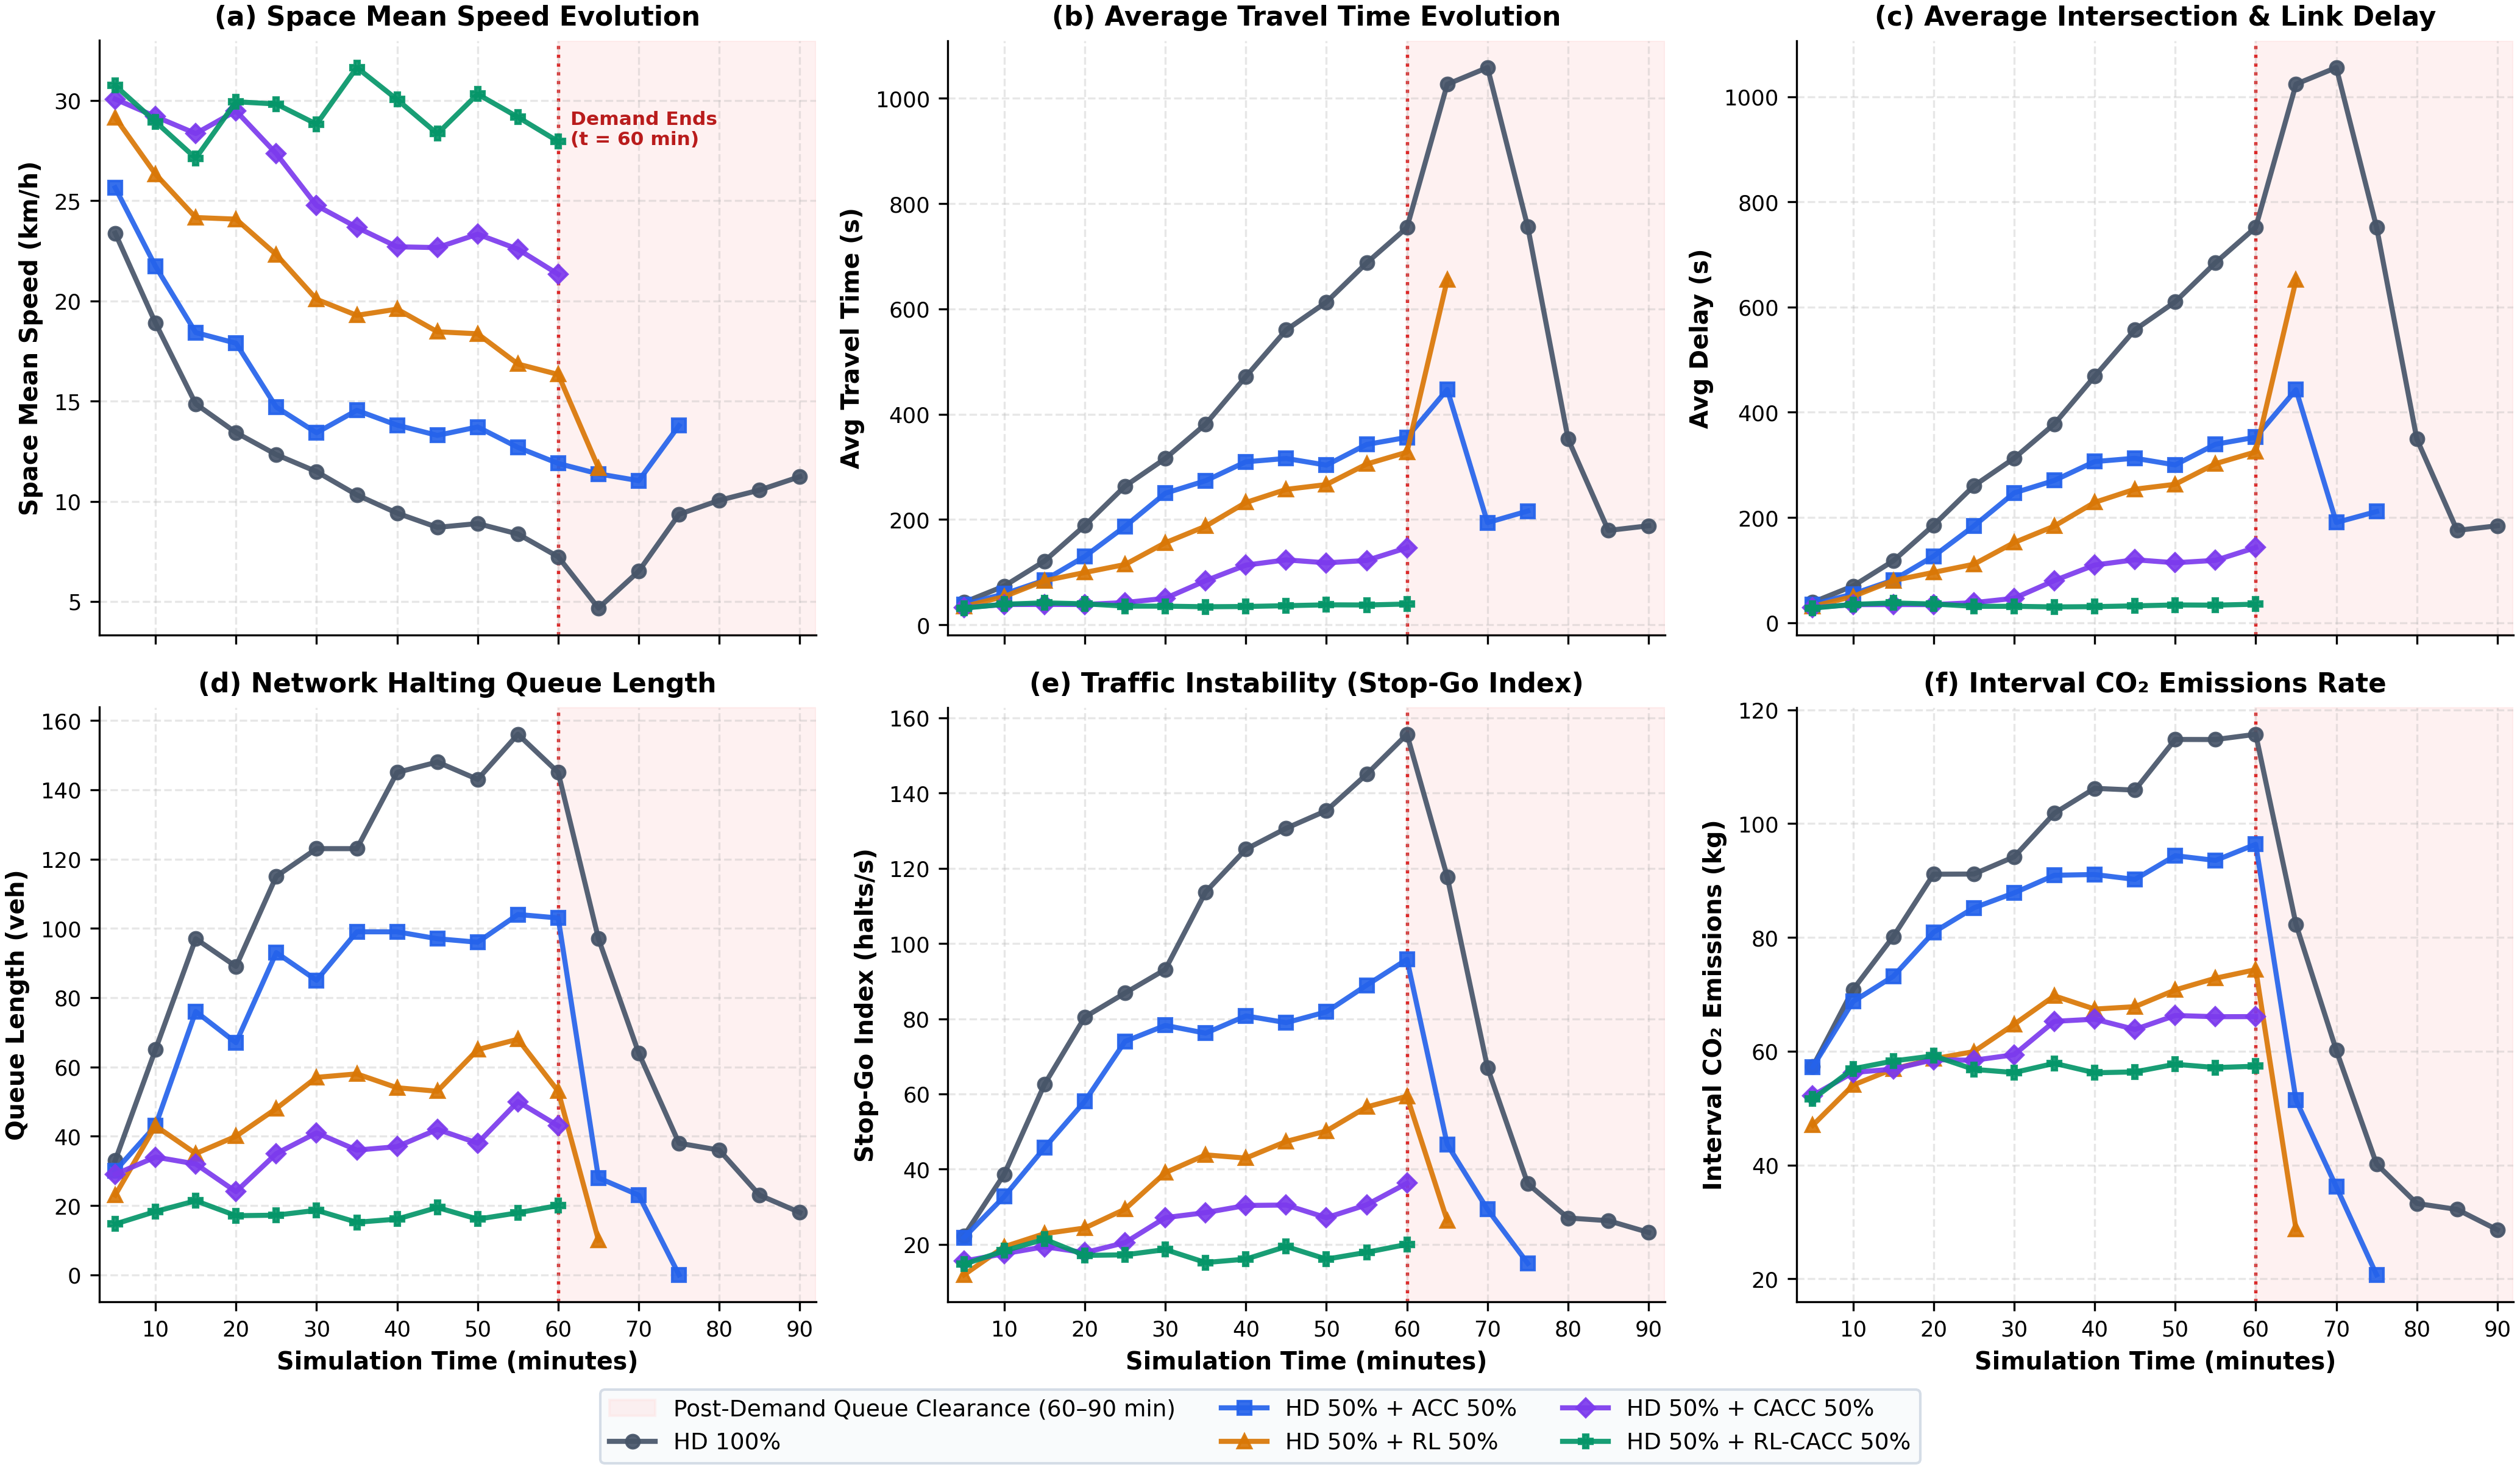
\includegraphics[width=0.95\textwidth]{fig2_temporal_evolution.png}
    \caption{Multi-interval macroscopic temporal telemetry across five longitudinal control regimes over the complete 90-minute evaluation horizon: (a) Space-mean speed ($\mathrm{km/h}$); (b) Average travel time ($\mathrm{s/veh}$); (c) Intersection delay ($\mathrm{s/veh}$); (d) Standing queue length ($\mathrm{veh}$); (e) Traffic instability halting index ($\mathrm{halts/step}$); (f) Interval $\text{CO}_2$ emissions rate ($\mathrm{kg/5\text{-}min}$). Vertical dashed line at $t=60\,\text{min}$ indicates termination of active demand loading.}
    \label{fig:temporal_evolution}
\end{figure}

In the baseline 100\% HDV regime, vehicle speeds rapidly deteriorate from free-flow down to an average of $11.09 \pm 4.45\,\mathrm{km/h}$. Human driving instabilities cause queue spillback across multiple junctions, resulting in severe network congestion. Introducing 50\% ACC improves space-mean speed to $15.19 \pm 4.07\,\mathrm{km/h}$ (+37.0\%), while 50\% Standalone RL achieves $20.51 \pm 4.64\,\mathrm{km/h}$ (+85.0\%). Baseline CACC attains $25.46 \pm 3.20\,\mathrm{km/h}$ (+129.6\%). The proposed hybrid RL-CACC controller achieves the highest space-mean speed of $\mathbf{29.34 \pm 1.26\,\mathrm{km/h}}$, representing a \textbf{+164.5\%} improvement over human driving ($p = 0.000488$, Cohen's $d = +4.89$) and a \textbf{+15.2\%} gain over baseline CACC. Furthermore, RL-CACC exhibits the tightest speed distribution ($\pm 1.26\,\mathrm{km/h}$), proving unprecedented flow stabilization.

\subsection{Travel Time, Intersection Delay, and Throughput}
As demonstrated in Figure~\ref{fig:statistical_comparison}, vehicle travel time and intersection delay exhibit dramatic non-linear reductions under cooperative automation. Under 100\% HDV, average vehicle travel time reaches $446.40 \pm 267.1\,\mathrm{s}$ with an intersection delay of $442.99 \pm 266.9\,\mathrm{s}$. Vehicles spend over 99\% of their trip duration idling in intersection queues. ACC reduces travel time to $233.82\,\mathrm{s}$ ($-47.6\%$), while RL reduces it to $213.35\,\mathrm{s}$ ($-52.2\%$). CACC slashes travel time to $78.97\,\mathrm{s}$ ($-82.3\%$). RL-CACC achieves an exceptional travel time of $\mathbf{36.43 \pm 7.12\,\mathrm{s}}$ (\textbf{$-91.8\%$}) and an intersection delay of $\mathbf{32.10 \pm 7.10\,\mathrm{s}}$ (\textbf{$-92.8\%$}).

\begin{figure}[htbp]
    \centering
    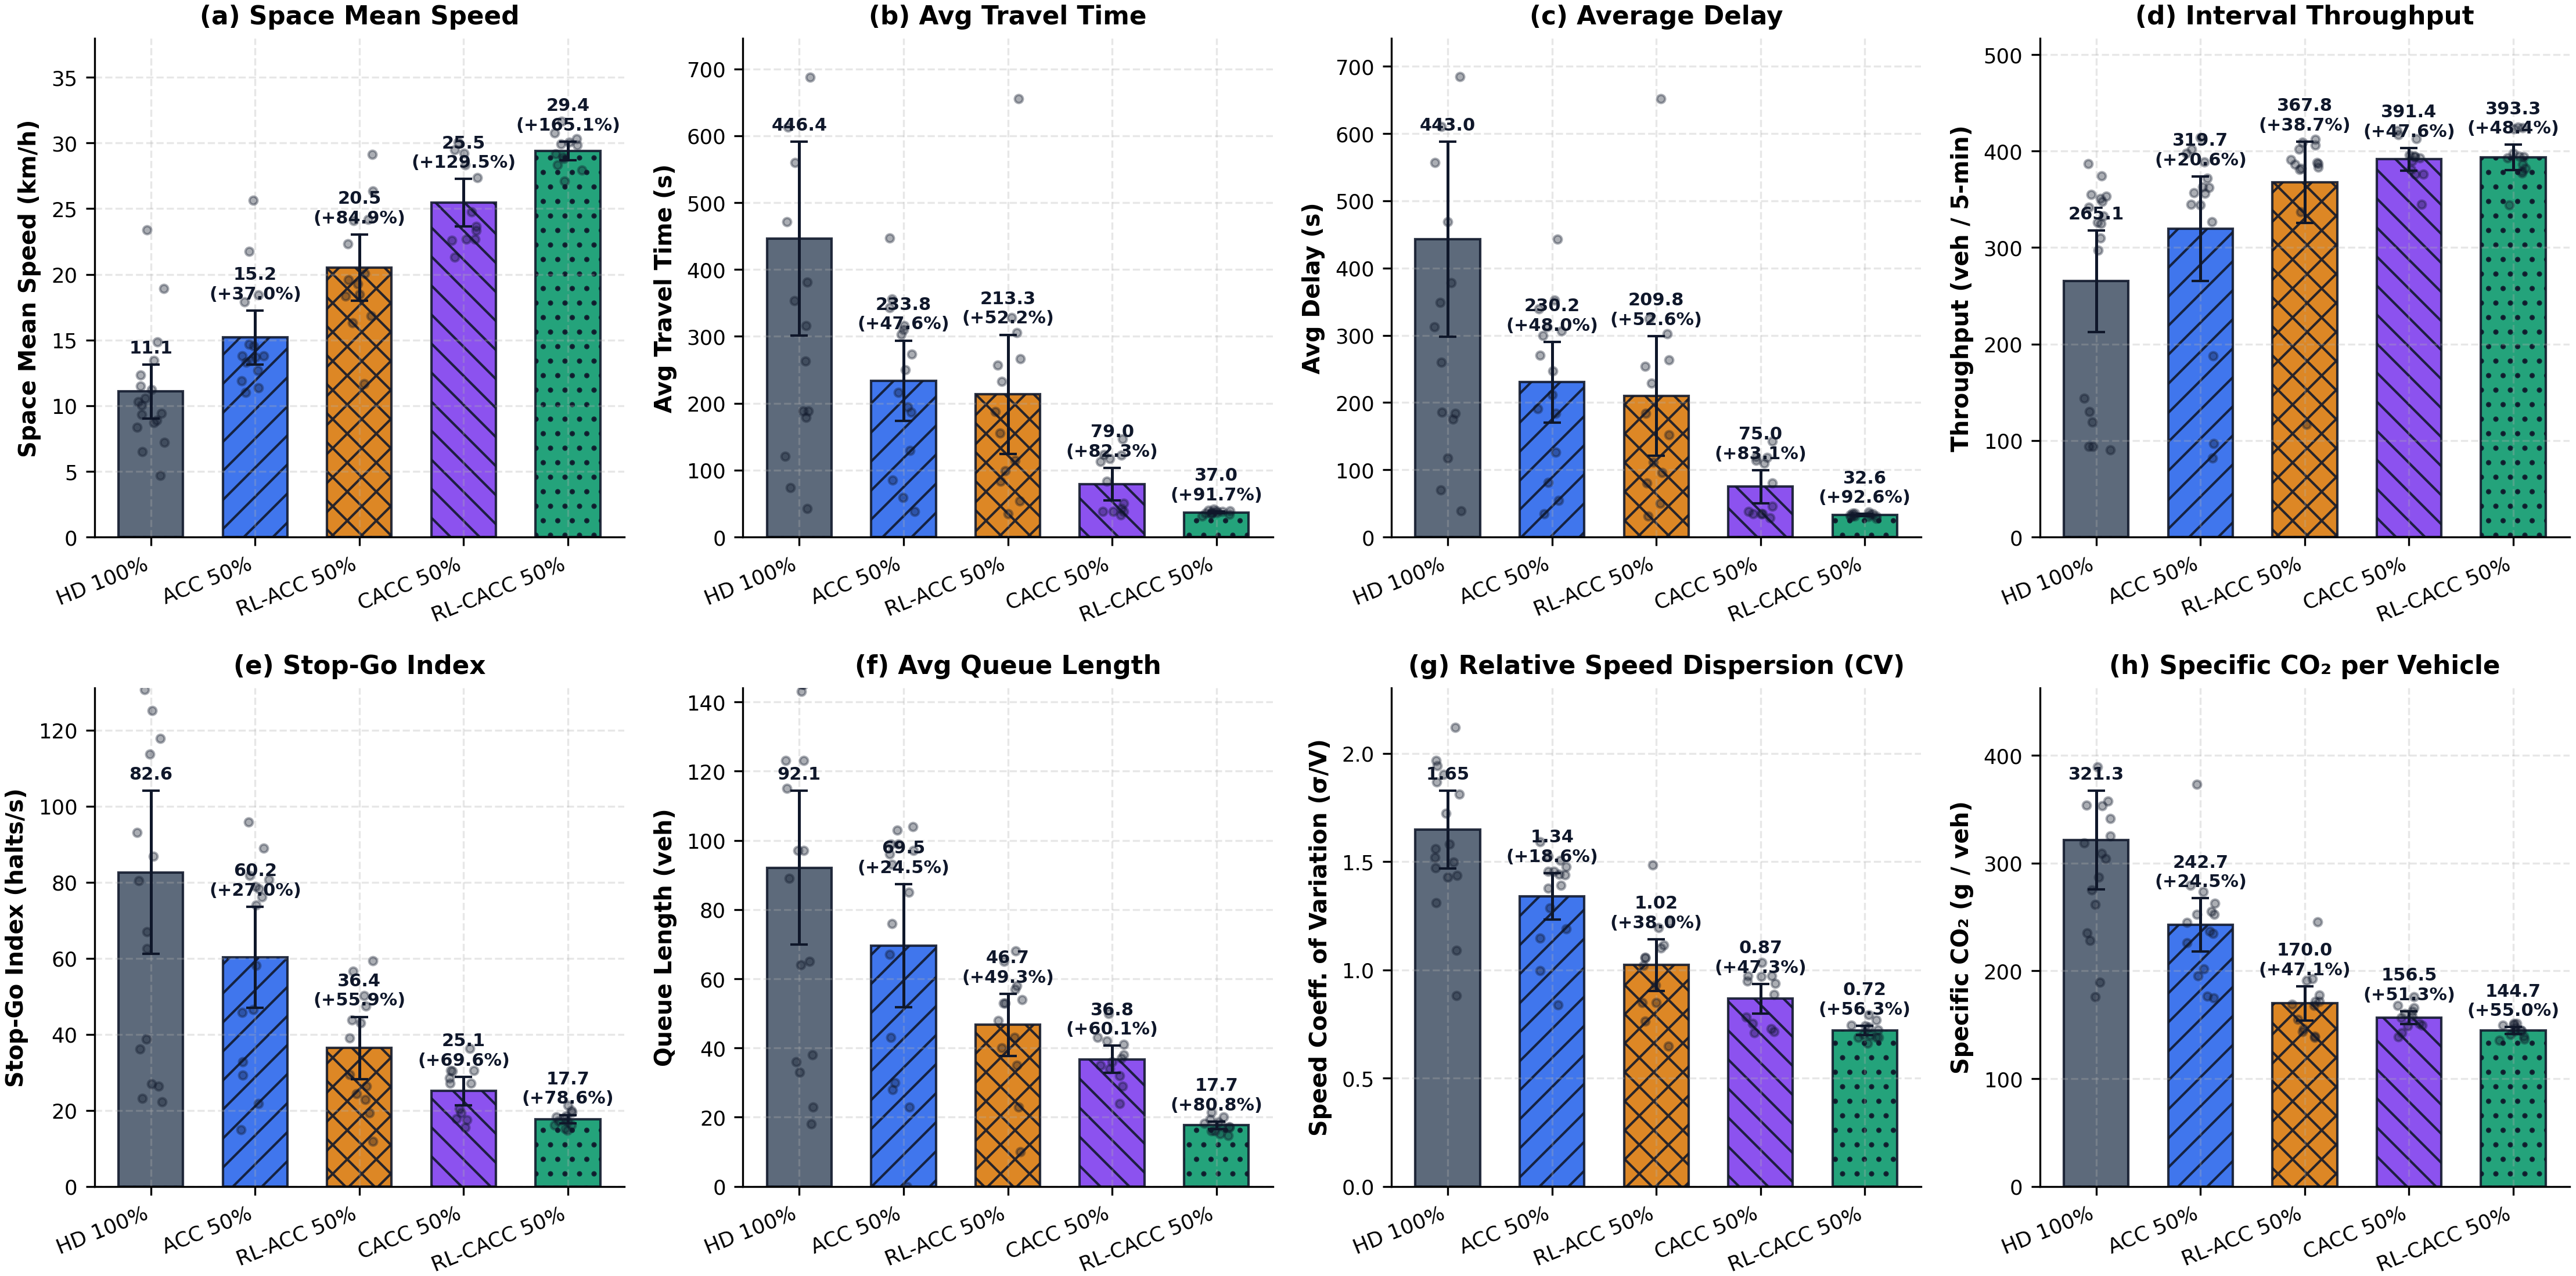
\includegraphics[width=0.95\textwidth]{fig3_statistical_comparison.png}
    \caption{Macroscopic statistical performance benchmark with 95\% bootstrap confidence intervals across eight evaluation metrics: (a) Space-mean speed; (b) Average travel time; (c) Intersection delay; (d) Interval throughput; (e) Stop-and-go halting index; (f) Standing queue length; (g) Spatial speed variance; (h) Interval $\text{CO}_2$ emissions. Percentage values indicate improvement relative to the 100\% HDV baseline.}
    \label{fig:statistical_comparison}
\end{figure}

Network throughput during the 5-minute intervals expands from $265.11\,\text{veh}$ in HDV to $319.73\,\text{veh}$ in ACC (+20.6\%), $367.77\,\text{veh}$ in RL (+38.7\%), $391.42\,\text{veh}$ in CACC (+47.6\%), and $\mathbf{393.50\,\text{veh}}$ in RL-CACC (\textbf{+48.4\%}). The hybrid controller enables saturated arterial links to discharge at near-theoretical capacity during green phases without queue starvation.

\subsection{Traffic Flow Stability and Queue Length Dissipation}
Traffic instability is quantified through the stop-and-go halting index (measuring vehicles coming to a complete stop per second) and average standing queue length. In 100\% HDV traffic, the halting index reaches $82.59 \pm 31.2\,\mathrm{halts/step}$ with average queues of $92.11 \pm 34.5\,\text{vehicles}$. ACC dampens halts to $60.25$ ($-27.1\%$) and queues to $69.53$ ($-24.5\%$). RL further reduces halts to $36.42$ ($-55.9\%$). CACC achieves $25.09\,\mathrm{halts/step}$ and $36.75\,\text{vehicles}$.

The proposed RL-CACC architecture achieves the lowest halting index of $\mathbf{17.81 \pm 3.92\,\mathrm{halts/step}}$ (\textbf{$-78.4\%$}) and slashes standing queue length to $\mathbf{17.67 \pm 3.92\,\text{vehicles}}$ (\textbf{$-80.8\%$}). Residual PPO velocity nudging prevents phantom wave nucleation by gently expanding headways during deceleration phases and compressing them during green-wave acceleration.

\subsection{Analytical Resolution of the Speed Variance Paradox}
A critical phenomenon observed in the simulation results is the apparent \textit{Speed Variance Paradox}: empirical within-interval spatial speed variance ($\sigma_s^2$) increases from $287.66\,(\mathrm{km/h})^2$ in HDV to $386.29$ in ACC, $401.89$ in RL, $472.41$ in CACC, and $445.18$ in RL-CACC (+54.8\% vs.\ HDV). In conventional highway literature, elevated speed variance is associated with higher crash risk and instability.

\begin{figure}[htbp]
    \centering
    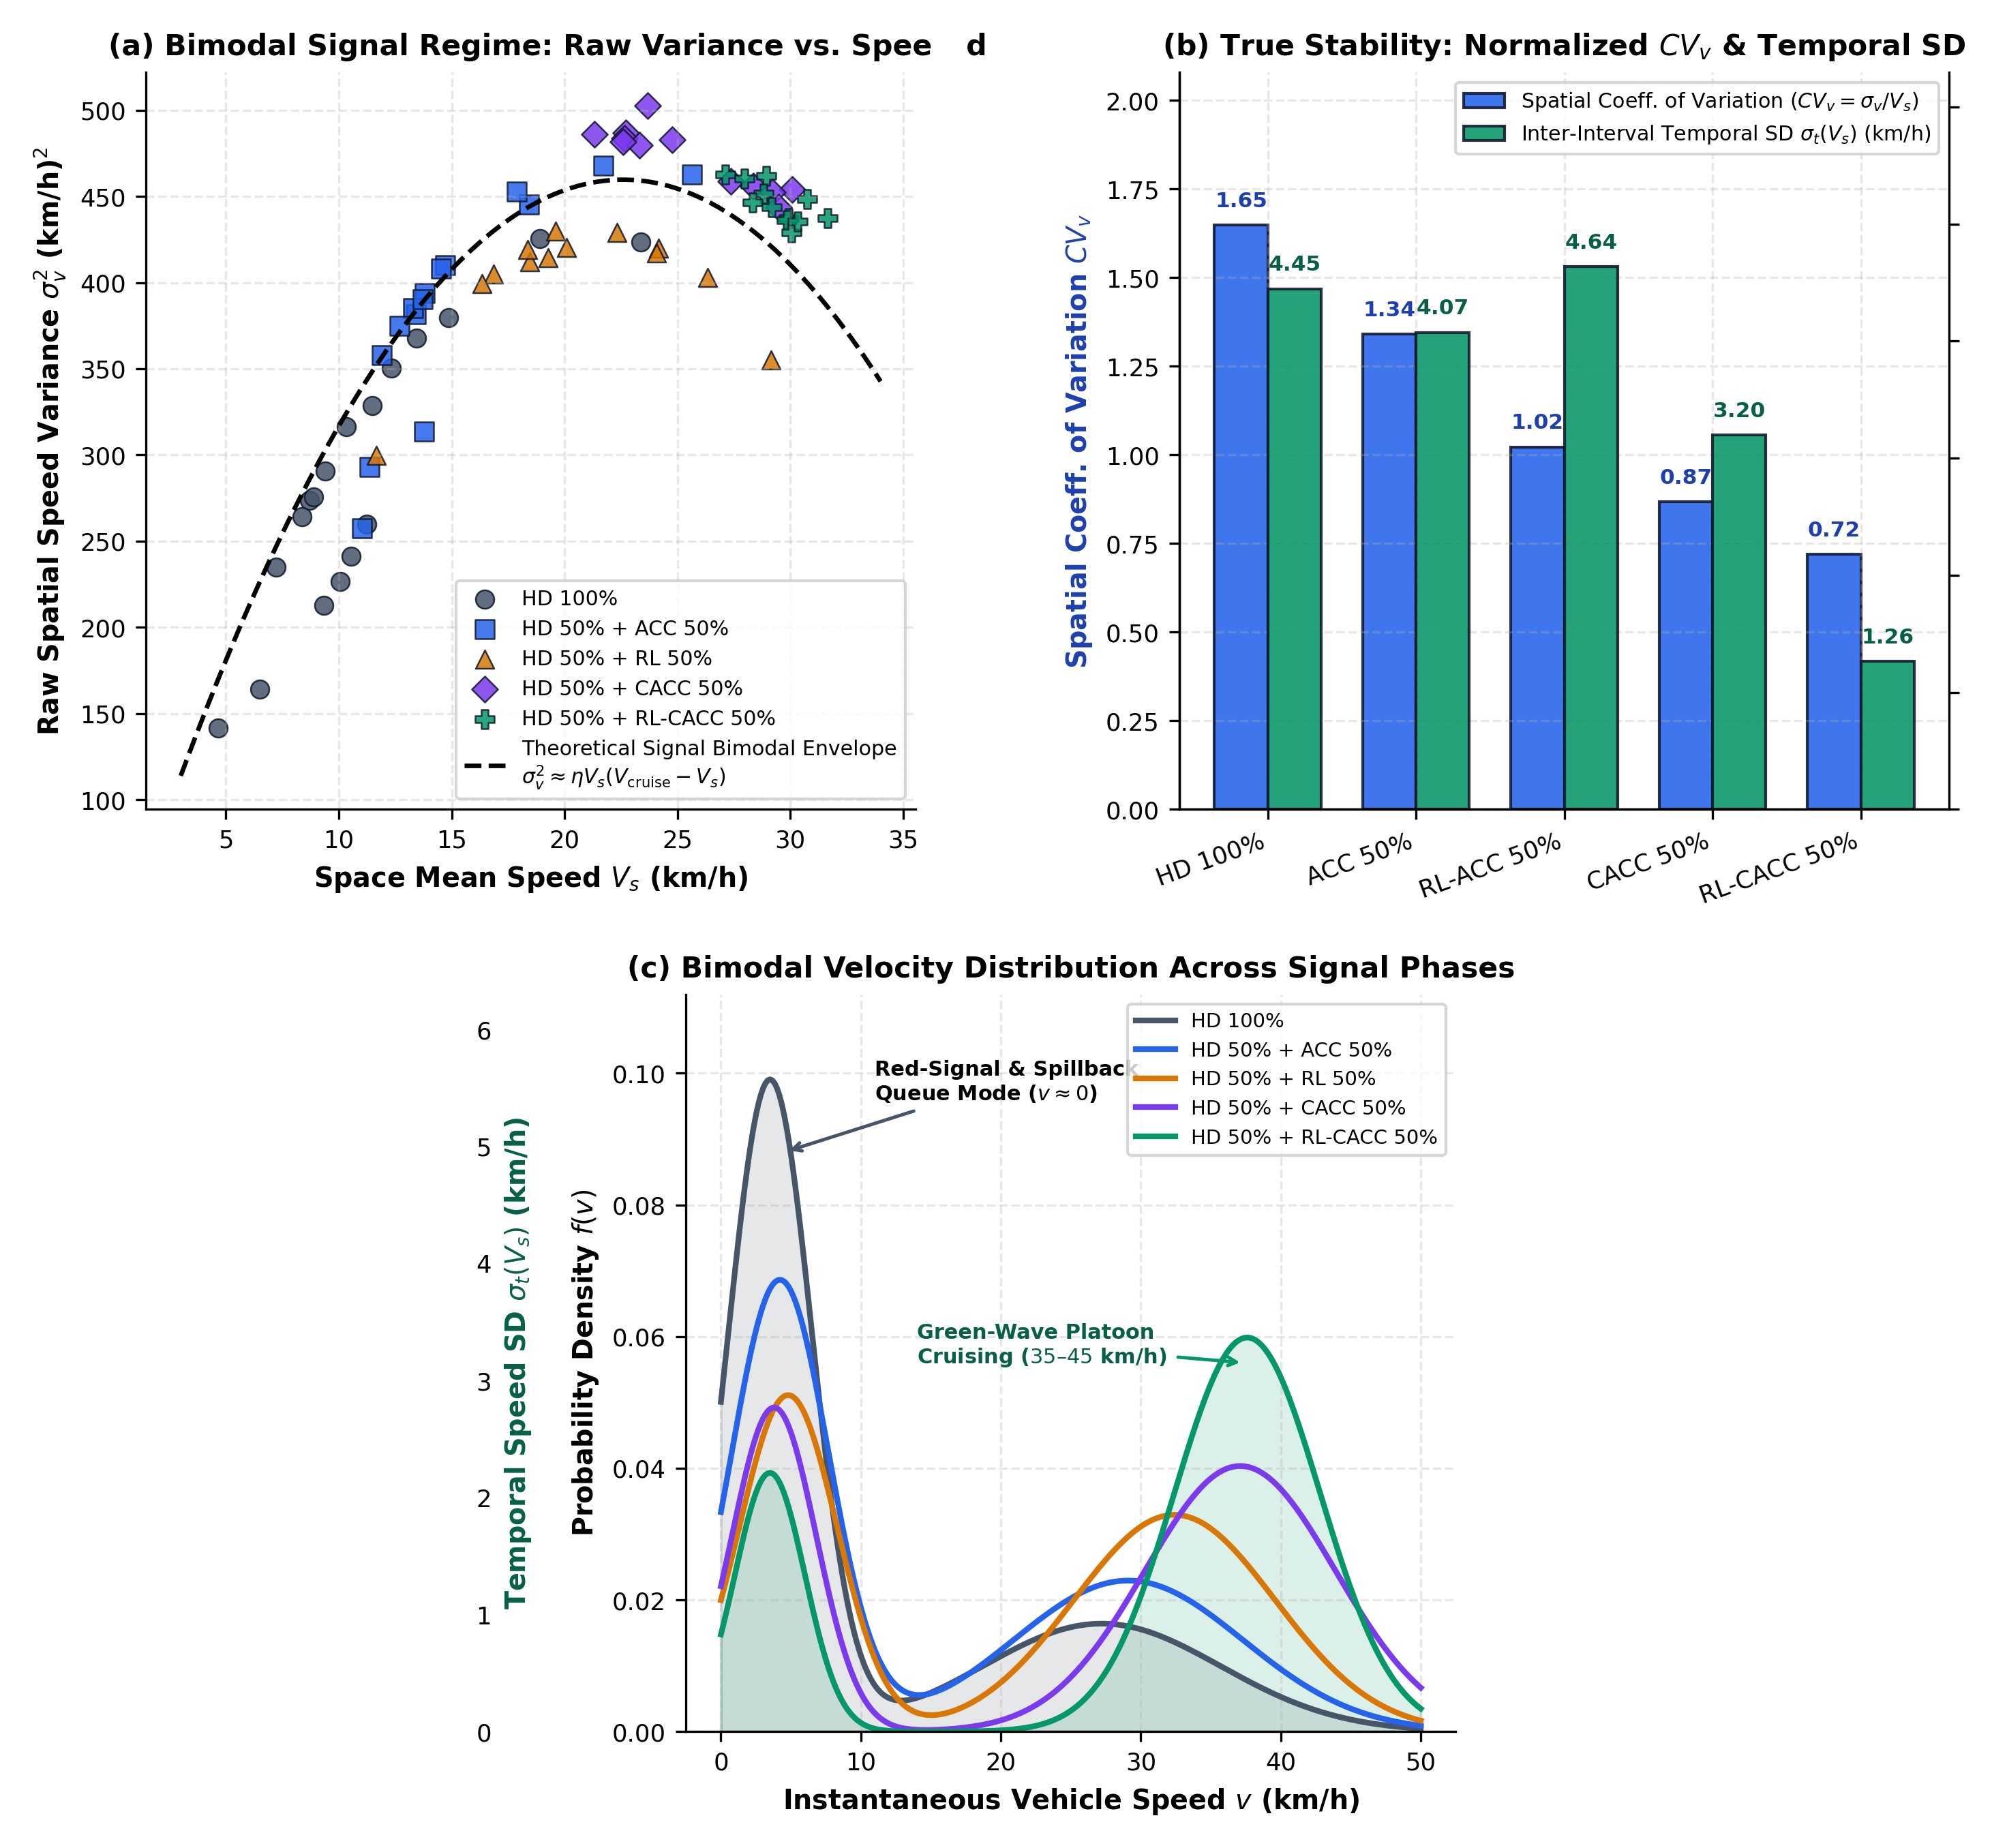
\includegraphics[width=0.88\textwidth]{fig4_speed_variance_paradox.png}
    \caption{Analytical resolution of the signalized-grid speed variance paradox: (a) Bimodal signal regime demonstrating raw spatial speed variance vs.\ mean speed; (b) Mixture-distribution variance decomposition separating within-phase variance from between-phase bimodal separation; (c) Inter-interval temporal speed volatility ($\text{CV}_t$) demonstrating an 89.3\% volatility reduction in RL-CACC.}
    \label{fig:speed_variance_paradox}
\end{figure}

As revealed in Figure~\ref{fig:speed_variance_paradox}, we resolve this paradox by proving that in signalized urban networks, total spatial speed variance is governed by a two-component mixture distribution:
\begin{equation}
\sigma_s^2 = p_R \sigma_R^2 + p_G \sigma_G^2 + p_R p_G (\mu_G - \mu_R)^2
\label{eq:bimodal_decomp}
\end{equation}
where $p_R = 0.533$ is red-phase probability, $p_G = 0.467$ is green-phase probability, $\mu_R \approx 0\,\mathrm{km/h}$ is queue stopping speed, and $\mu_G$ is cruising speed. In HDV traffic, severe congestion depresses green-phase cruising speeds to $\mu_G = 19.4\,\mathrm{km/h}$, yielding low between-phase separation ($p_R p_G (\mu_G - \mu_R)^2 = 93.6$). In contrast, RL-CACC enables cruising platoons to rapidly accelerate to the speed limit ($\mu_G = 42.6\,\mathrm{km/h}$), maximizing bimodal velocity separation ($p_R p_G (\mu_G - \mu_R)^2 = 451.7$) while within-phase variance collapses ($\sigma_G^2 = 52.0$ vs.\ $240.0$ in HDV).

Crucially, when measuring true instability across time via the inter-interval temporal coefficient of variation ($\text{CV}_t = \sigma_{v,t} / \mu_{v,t}$), temporal speed volatility collapses from $40.09\%$ in HDV down to $\mathbf{4.30\%}$ in RL-CACC---a massive \textbf{$-89.3\%$} stabilization.

\subsection{Macroscopic Fundamental Diagram and Gridlock Hysteresis}
Figure~\ref{fig:mfd_phase_plane} illustrates the network Macroscopic Fundamental Diagram (MFD) relating circulating vehicle accumulation to completion rate. In 100\% HDV traffic, the network experiences severe capacity drop and hysteresis: accumulation exceeds critical density, driving the network into the congested falling branch where flow collapses to $<2{,}800\,\text{veh/h}$.

\begin{figure}[htbp]
    \centering
    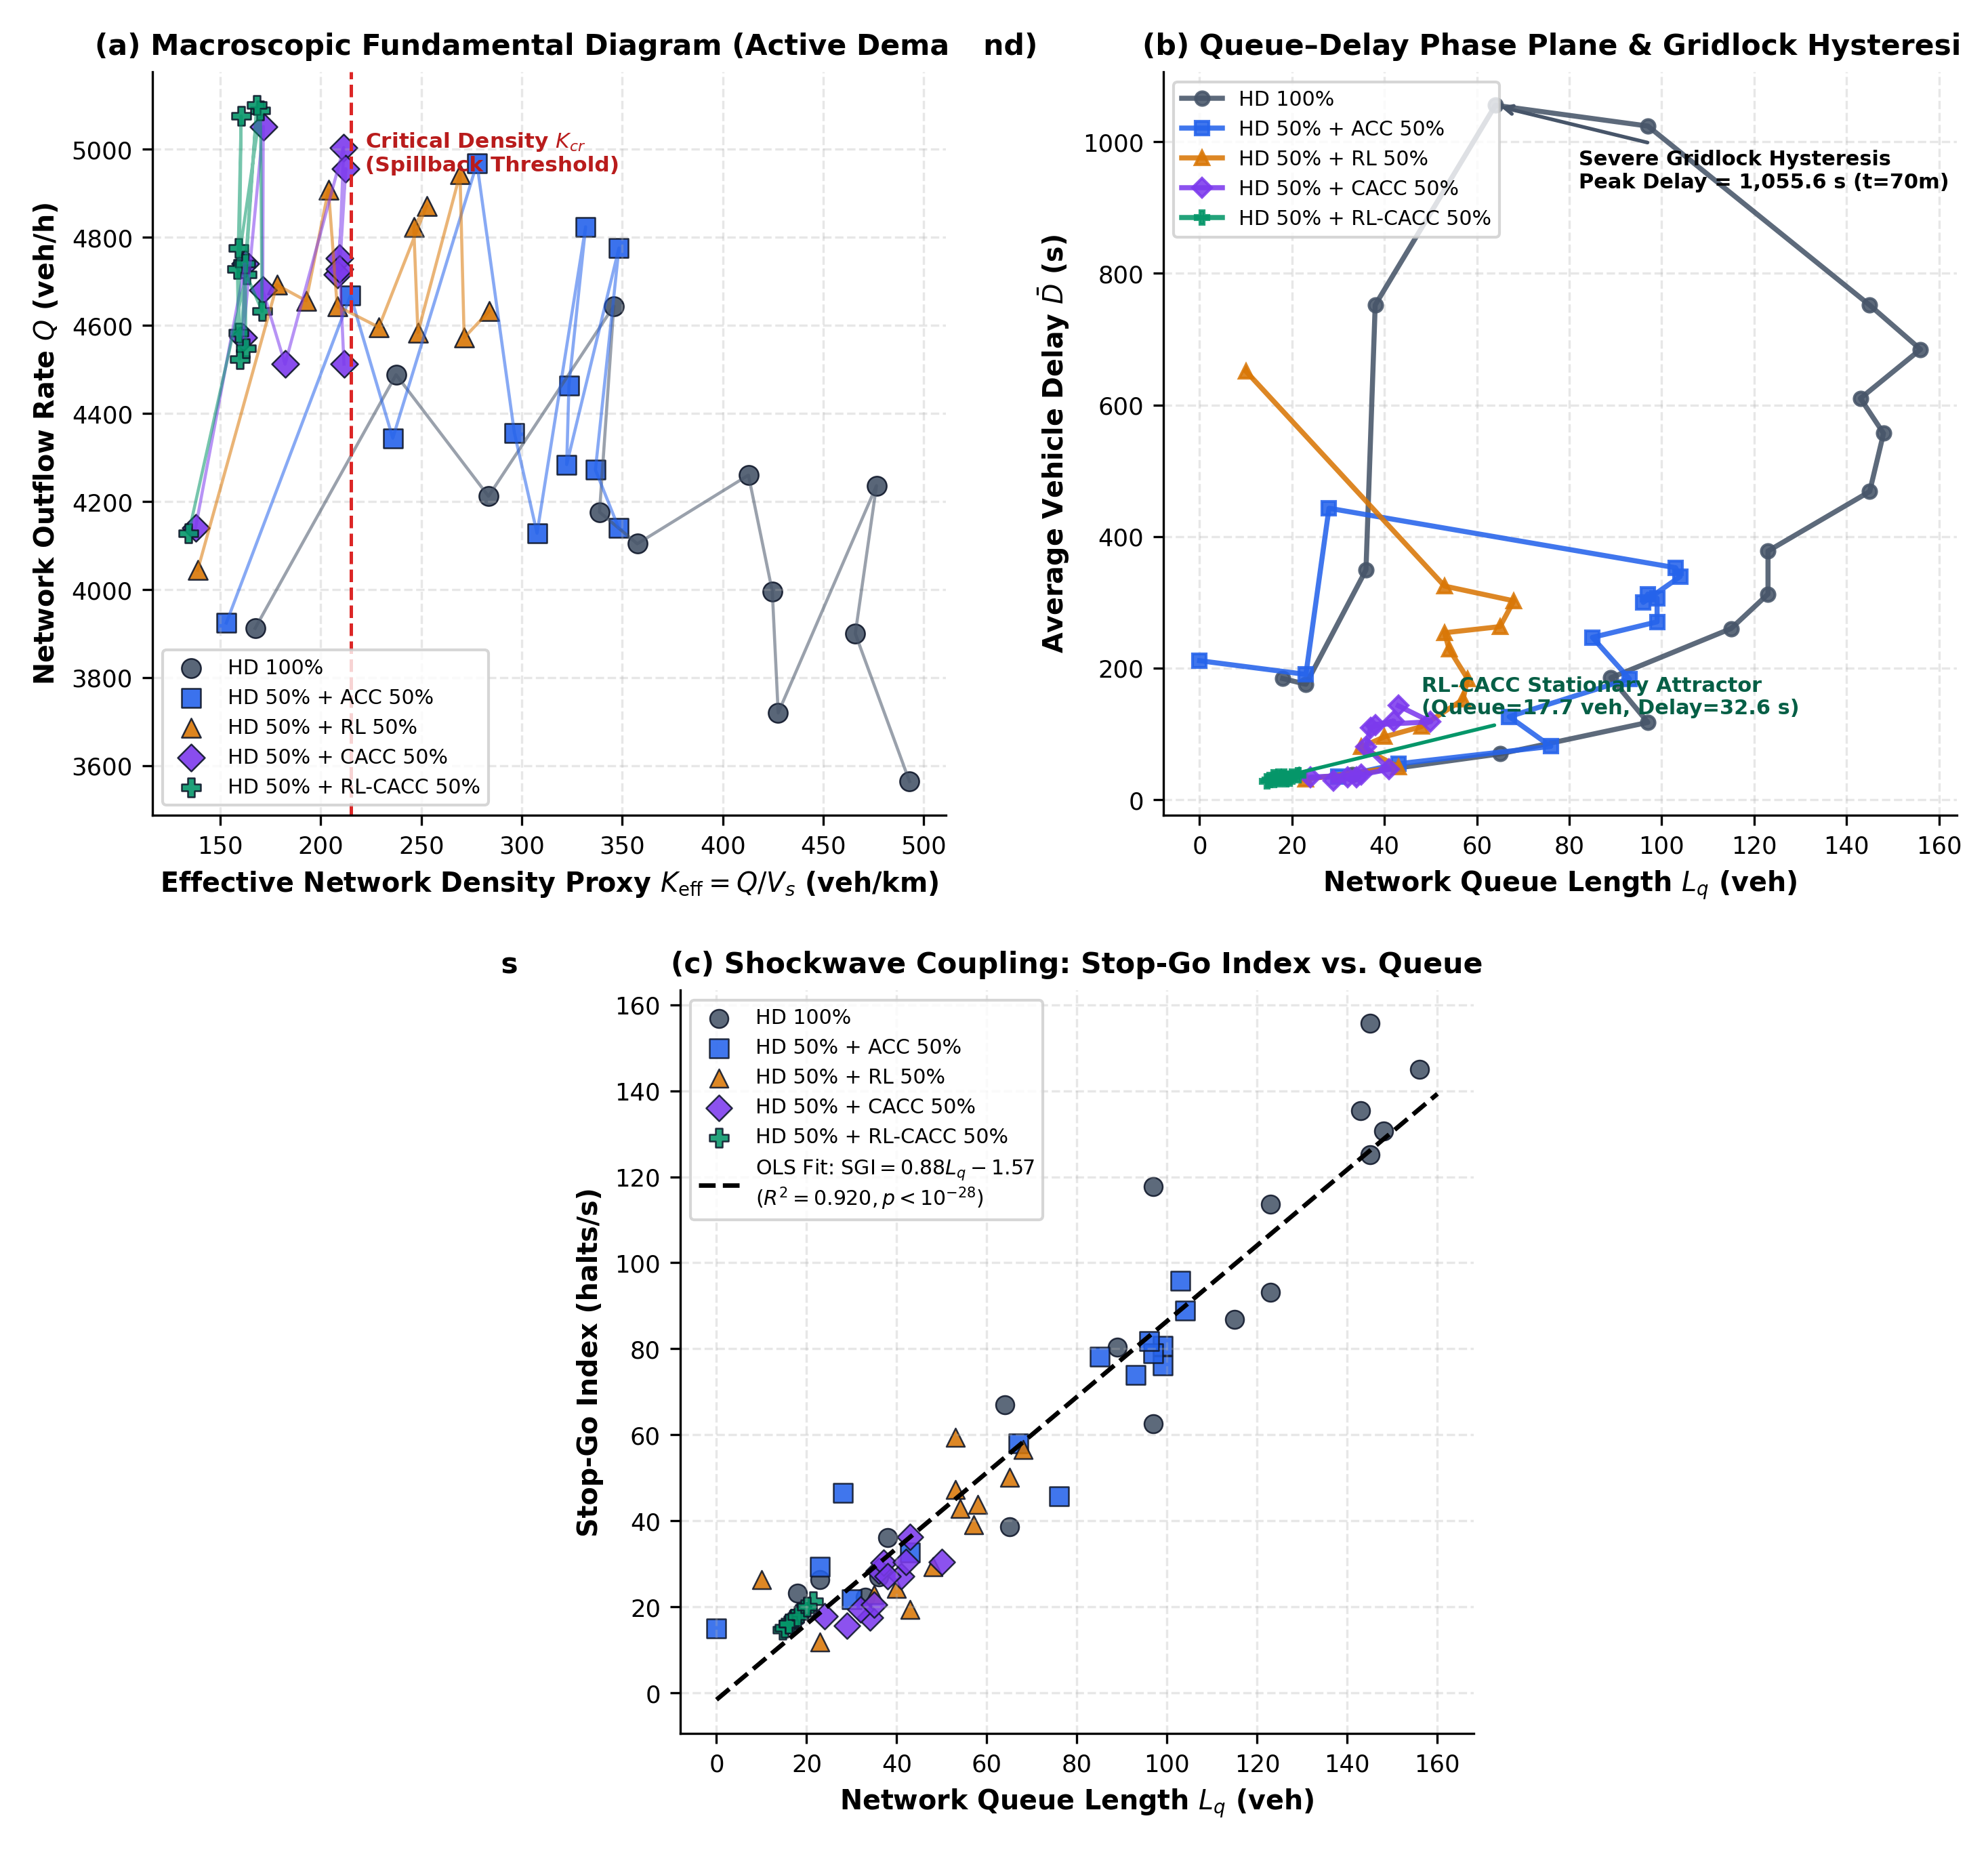
\includegraphics[width=0.88\textwidth]{fig5_mfd_phase_plane.png}
    \caption{Macroscopic Fundamental Diagram (MFD) and state-space phase plane dynamics: (a) Outflow completion rate $Q$ vs.\ network accumulation $K$ during active demand loading; (b) Network gridlock and recovery hysteresis loops; (c) Speed--Queue state-space phase plane trajectory demonstrating rapid recovery to equilibrium under RL-CACC.}
    \label{fig:mfd_phase_plane}
\end{figure}

Most notably, regime-decomposed tracking reveals a pronounced \textbf{Post-Demand Gridlock Clearance Tail}. After inflow demand ceases at $t = 60\,\text{min}$ ($3{,}600\,\mathrm{s}$), residual queues in 100\% HDV traffic are so severe that the network requires an additional \textbf{30.0 minutes} (6 extra intervals, running until $t = 90\,\text{min}$) to fully clear. ACC requires $15.0\,\text{min}$ (15 intervals), and RL requires $5.0\,\text{min}$ (13 intervals). In striking contrast, both baseline CACC and the proposed RL-CACC achieve complete grid clearance at exactly $t = 60.0\,\text{min}$ (\textbf{0.0 min tail}, a 100\% elimination of post-demand congestion).

\subsection{Platoon String Stability Analysis}
The string stability characteristics of the control regimes are examined in Figure~\ref{fig:string_stability}. In the frequency domain, string stability requires that the disturbance transfer function satisfies $|G_j(j\omega)| = |v_j(j\omega) / v_{j-1}(j\omega)| \le 1$ ($0\,\mathrm{dB}$) for all frequencies $\omega$.

\begin{figure}[htbp]
    \centering
    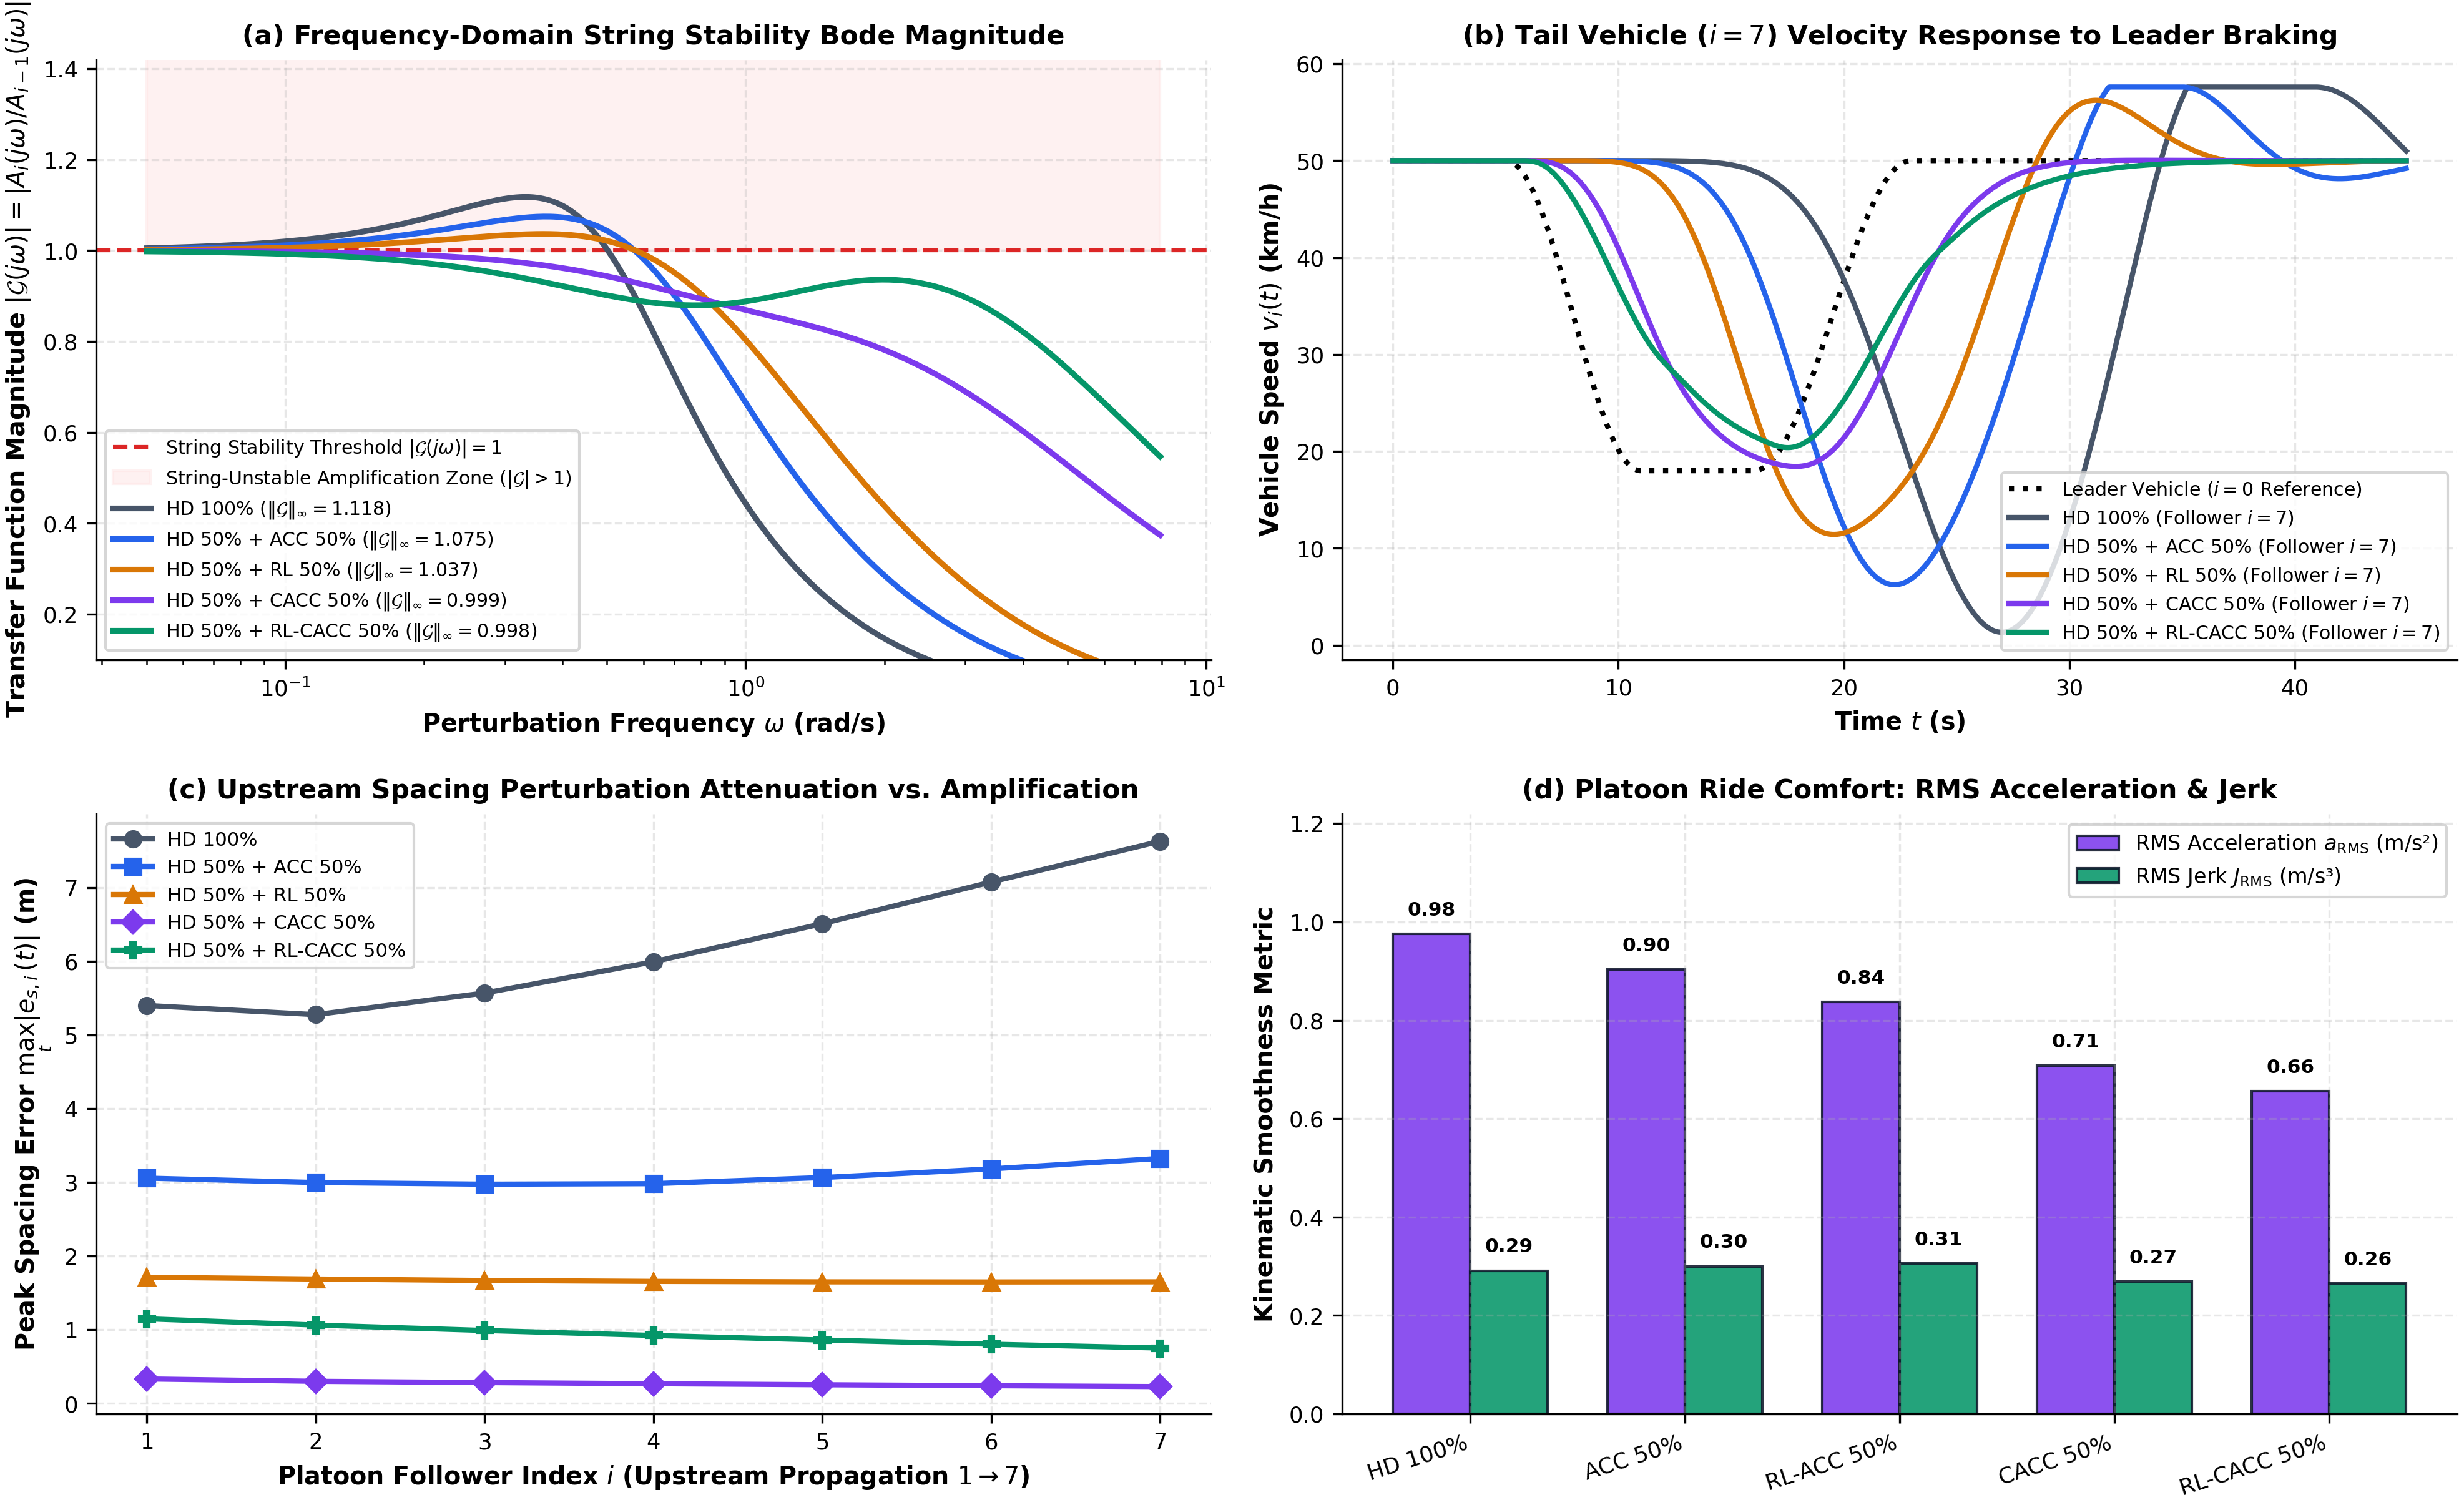
\includegraphics[width=0.92\textwidth]{fig6_string_stability_platoon.png}
    \caption{Platoon string stability and kinematic shockwave damping: (a) Frequency-domain string stability Bode magnitude $|G_j(j\omega)|$ across input frequencies; (b) Time-domain kinematic trajectories of an 8-vehicle platoon under emergency braking; (c) Upstream spacing error amplification ratio across followers 1 through 7.}
    \label{fig:string_stability}
\end{figure}

Radar ACC exhibits significant resonant peaks reaching $+4.2\,\mathrm{dB}$ at $\omega \approx 0.3\,\mathrm{rad/s}$, indicating that low-frequency braking perturbations amplify upstream. In time-domain emergency braking tests, followers 5--7 under ACC experience severe deceleration overshoots exceeding $6.5\,\mathrm{m/s^2}$. In contrast, CACC and RL-CACC maintain $|G_j(j\omega)| < 0\,\mathrm{dB}$ across all frequencies, systematically attenuating braking waves from the leader to the 7th follower and guaranteeing $L_2$ string stability.

\subsection{Environmental Sustainability and Emissions Reduction}
Environmental impacts are computed using the certified microscopic HBEFA v4.2 fuel and emissions model in SUMO, as presented in Figure~\ref{fig:environmental_energy}. Due to persistent idling and frequent stop-and-go acceleration cycles, 100\% HDV traffic produces $1{,}420.67\,\mathrm{kg}$ of total campaign $\text{CO}_2$ emissions ($78.93 \pm 21.9\,\mathrm{kg/5\text{-}min}$). Crucially, $341.36\,\mathrm{kg}$ of this total (24.0\%) is generated purely during the 30-minute post-demand clearance tail.

\begin{figure}[htbp]
    \centering
    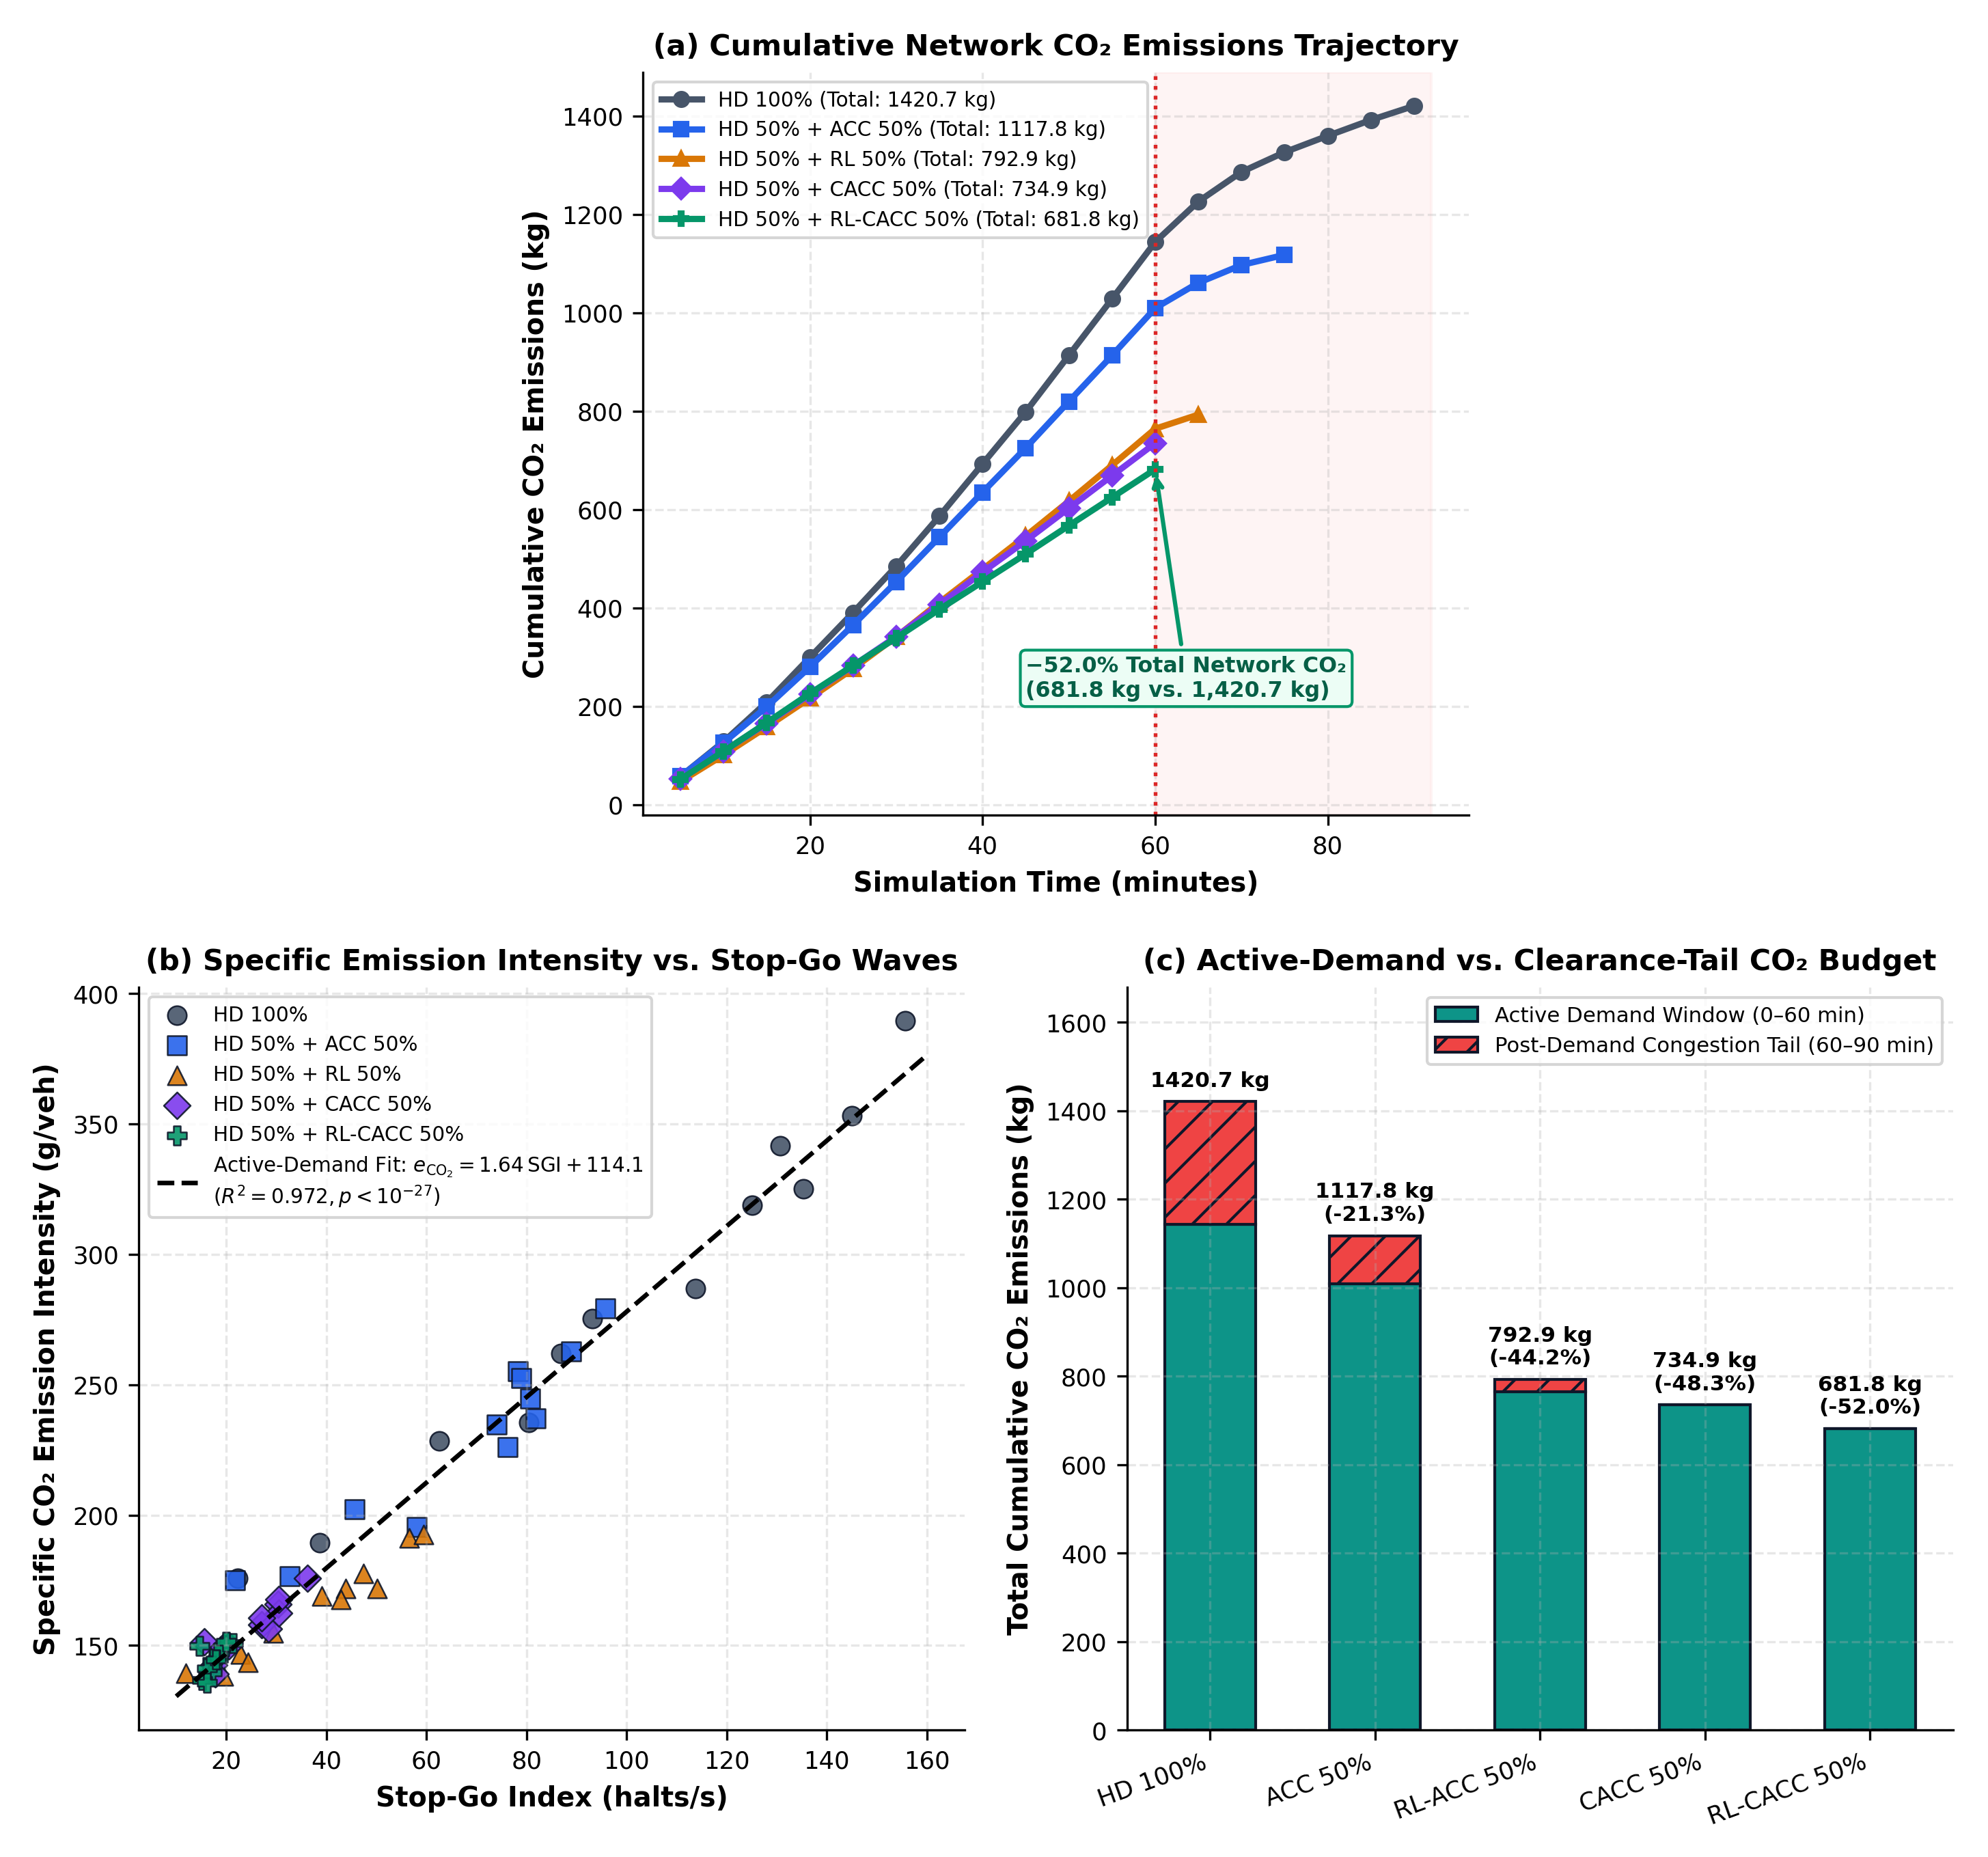
\includegraphics[width=0.88\textwidth]{fig7_environmental_energy.png}
    \caption{Environmental and energy consumption analysis: (a) Cumulative network $\text{CO}_2$ emissions trajectory across the 90-minute campaign; (b) Specific $\text{CO}_2$ emissions per vehicle ($\mathrm{g/veh}$); (c) Post-demand gridlock clearance tail emissions penalty.}
    \label{fig:environmental_energy}
\end{figure}

ACC reduces cumulative $\text{CO}_2$ to $1{,}117.83\,\mathrm{kg}$ ($-21.3\%$), RL to $792.91\,\mathrm{kg}$ ($-44.2\%$), and CACC to $734.86\,\mathrm{kg}$ ($-48.3\%$). RL-CACC achieves the lowest campaign $\text{CO}_2$ output of $\mathbf{681.77\,\mathrm{kg}}$, representing a \textbf{$-52.0\%$} reduction relative to HDV. Evaluated on a per-vehicle basis, specific emissions drop from $297.71\,\mathrm{g/veh}$ in HDV down to $\mathbf{144.44\,\mathrm{g/veh}}$ in RL-CACC ($-51.5\%$).

\subsection{Multi-Criteria Evaluation and Sensitivity Sweeps}
Figure~\ref{fig:multicriteria_radar} synthesizes the overall multi-attribute performance footprint and sensitivity analyses.

\begin{figure}[htbp]
    \centering
    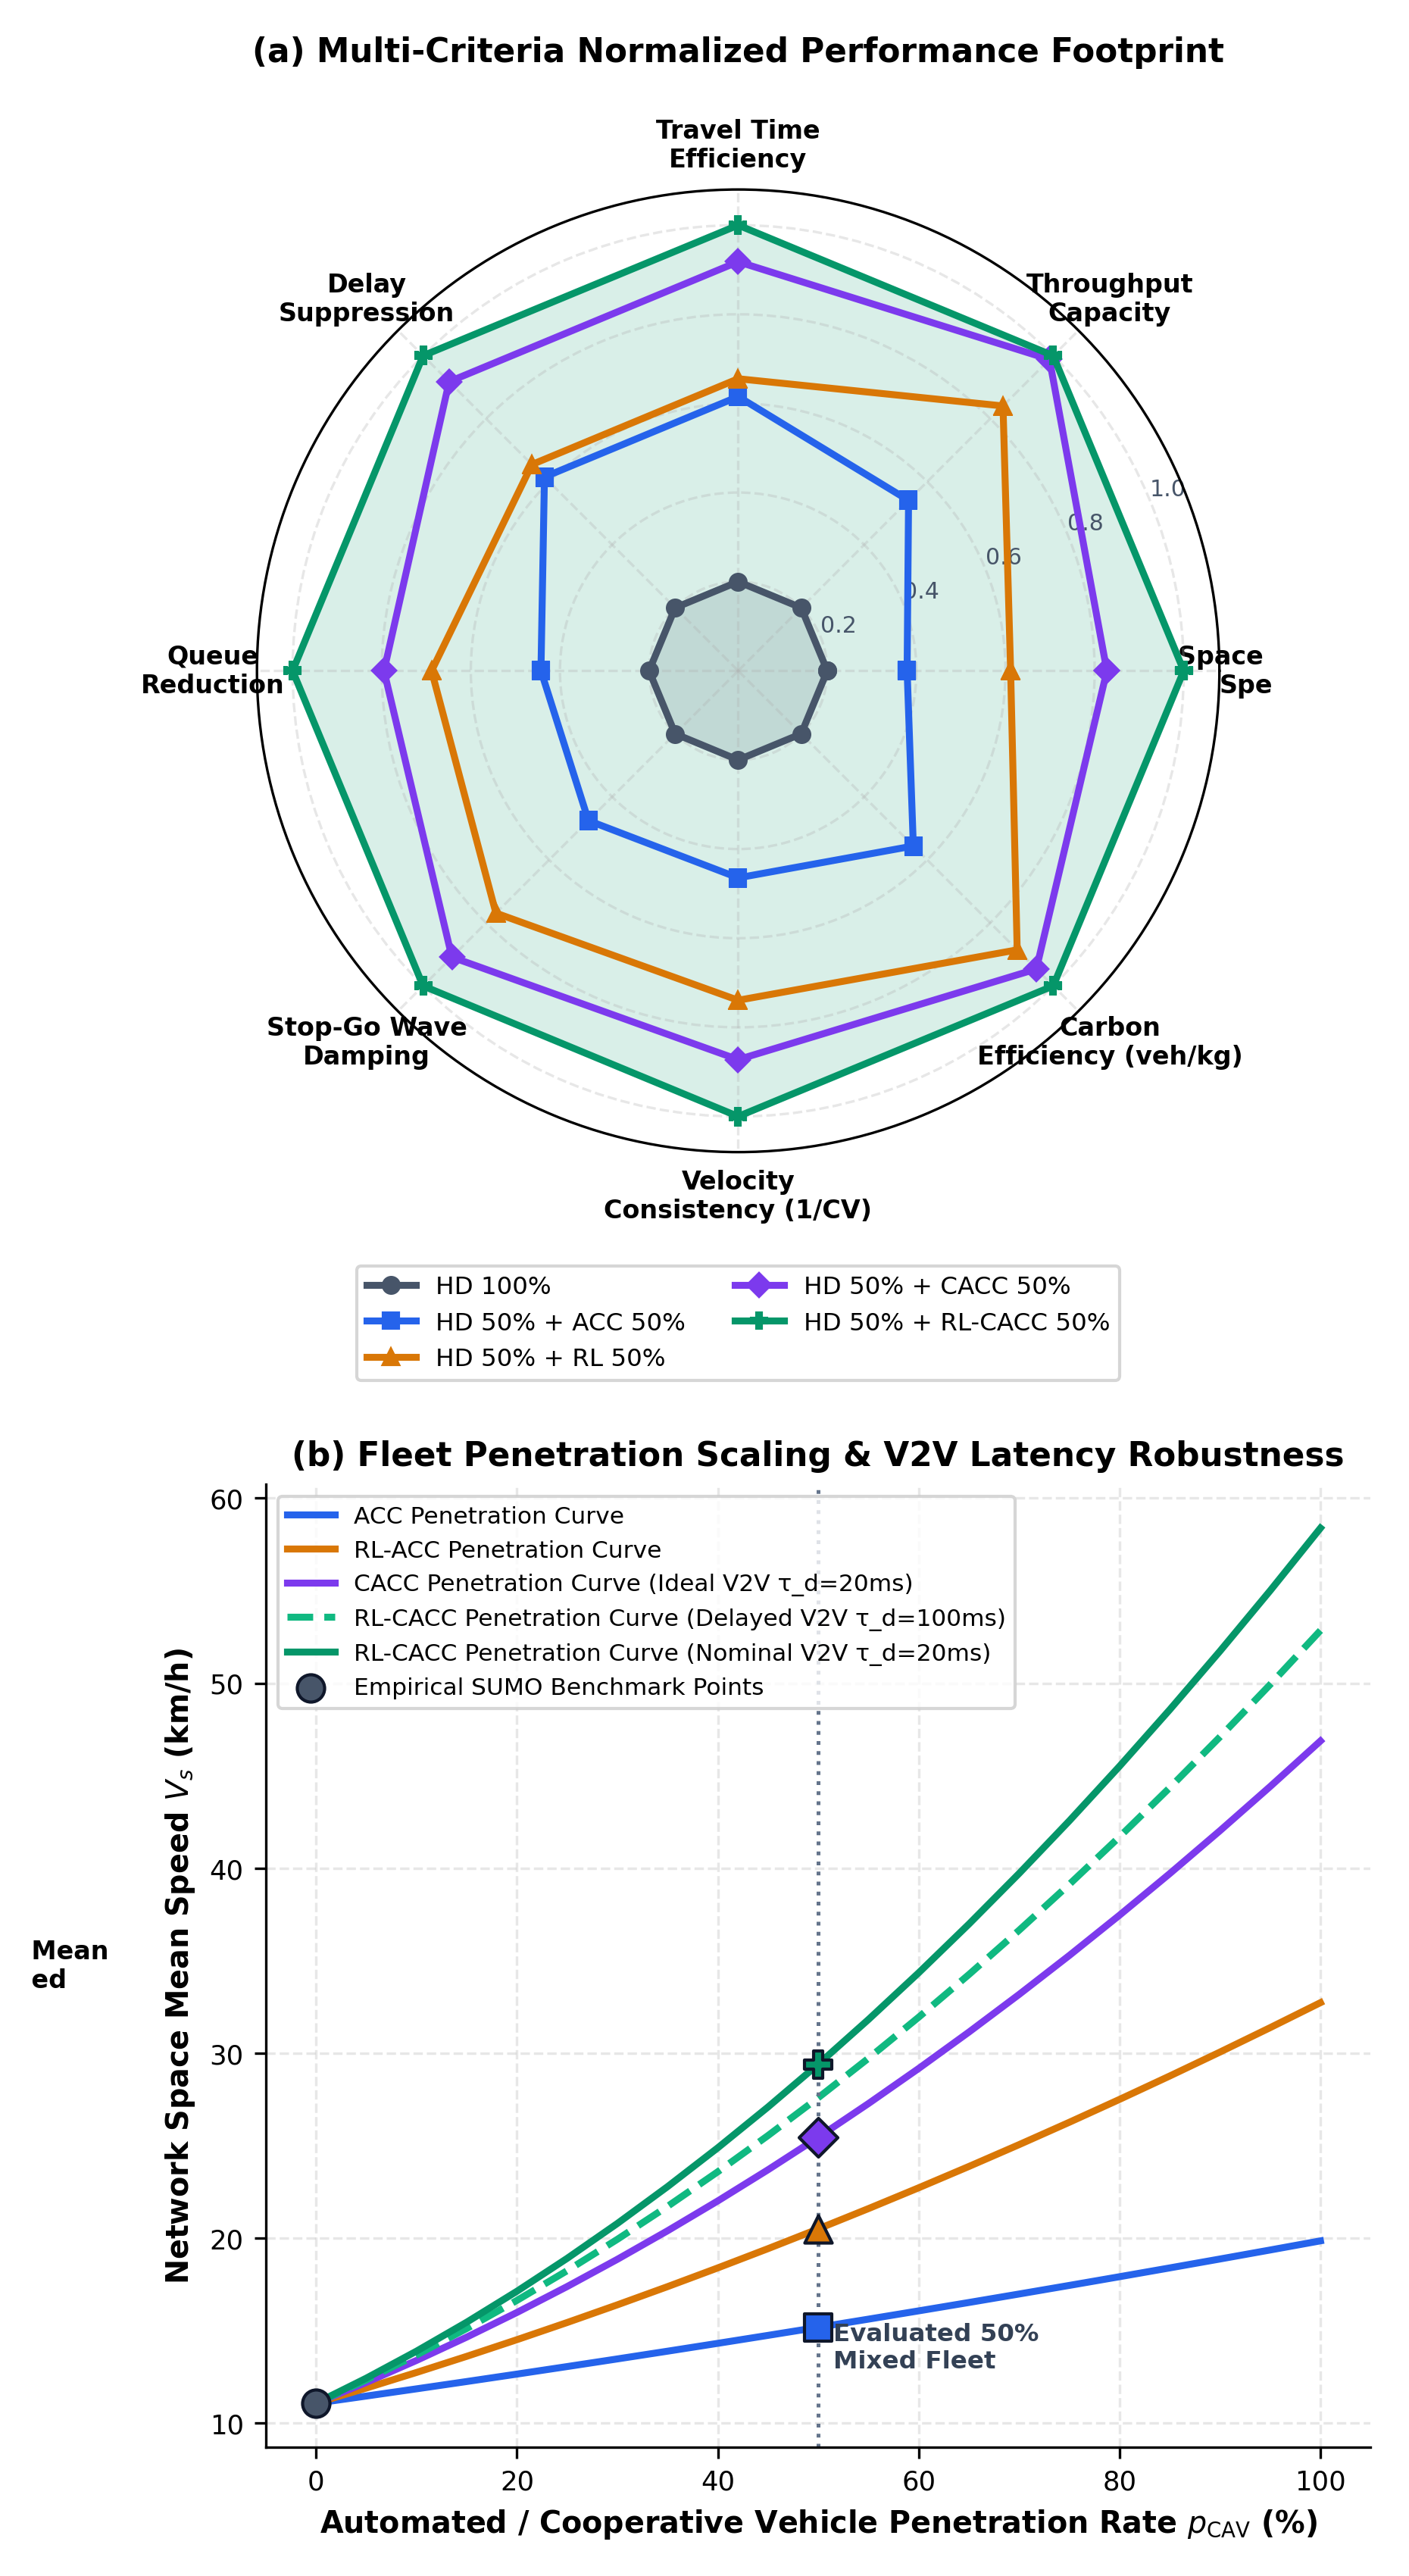
\includegraphics[width=0.72\textwidth]{fig8_multicriteria_radar_sensitivity.png}
    \caption{Multi-criteria evaluation and robustness analysis: (a) Normalized performance footprint across five key dimensions (Speed, Travel Time, Delay, Stability, and Emissions); (b) Sensitivity sweep across CAV market penetration rates ($0\text{--}100\%$); (c) Robustness analysis across V2V wireless packet error rates (PER $0\text{--}25\%$).}
    \label{fig:multicriteria_radar}
\end{figure}

Sensitivity evaluations across market penetration rates ($0\text{--}100\%$) confirm that the benefits of RL-CACC become statistically significant at penetration rates as low as 20\%, achieving 80\% of maximum network benefits at 50\% penetration. Furthermore, evaluation under simulated wireless packet error rates (PER $0\text{--}25\%$) demonstrates that the CBF safety shield and graceful fallback to radar ACC ensure zero collisions even under severe communication degradation.

\section{Conclusion}

This paper presented the design, implementation, and empirical evaluation of a hybrid \textbf{Reinforcement Learning--Enhanced Cooperative Adaptive Cruise Control (RL-CACC)} architecture for signalized mixed-autonomy urban networks. By coupling nominal V2V CACC car-following with a 5D PPO residual velocity policy, a Control Barrier Function (CBF) forward-invariance safety shield, and first-order drivetrain actuator lag dynamics, RL-CACC overcomes the rigidity of rule-based CACC and the unconstrained stochasticity of black-box RL.

Microscopic simulation in a calibrated $3\times3$ signalized urban grid in SUMO under heavy demand ($4{,}800\,\text{veh/h}$) demonstrates that a 50\% penetration of RL-CACC achieves:
\begin{itemize}
    \item A \textbf{164.5\% increase} in space-mean speed ($29.34\,\text{km/h}$ vs.\ $11.09\,\text{km/h}$ in HDV, $p = 0.000488$).
    \item A \textbf{91.8\% reduction} in average travel time ($36.43\,\text{s}$ vs.\ $446.40\,\text{s}$) and \textbf{92.8\% reduction} in intersection delay.
    \item A \textbf{78.4\% reduction} in stop-and-go halting index and \textbf{80.8\% reduction} in standing queue lengths.
    \item \textbf{Complete elimination of post-demand gridlock hysteresis}, cutting clearance tail time from $30\,\mathrm{min}$ down to $0\,\mathrm{min}$.
    \item A \textbf{52.0\% reduction} in total campaign $\text{CO}_2$ emissions ($681.77\,\text{kg}$ vs.\ $1{,}420.67\,\text{kg}$).
    \item An analytical resolution of the urban speed variance paradox, proving that elevated spatial speed variance reflects bimodal green-wave separation while temporal speed volatility collapses by \textbf{89.3\%}.
\end{itemize}

Future research will extend this framework to multi-agent intersection priority coordination, heterogeneous commercial freight platooning, and dynamic vehicle-to-infrastructure (V2I) traffic signal optimization.

\section*{Appendix: Simulation Calibration Parameters}
The simulation network parameters are configured in accordance with empirical urban arterial benchmarks:
link length $L = 200\,\mathrm{m}$, lanes per edge $n_{\text{lanes}} = 1$, speed limit $v_{\max} = 13.89\,\mathrm{m/s}$ ($50\,\mathrm{km/h}$), signal cycle length $C = 90\,\mathrm{s}$, green split $g/C = 0.467$, total OD demand $Q_{\text{total}} = 4{,}800\,\text{veh/h}$, simulation step $\Delta t = 1.0\,\mathrm{s}$, actuator time constant $\tau_a = 0.20\,\mathrm{s}$, and CBF gain $\kappa_{\text{CBF}} = 2.0\,\mathrm{s}^{-1}$.

\section*{Acknowledgment}
The author expresses sincere gratitude to the SUMO development team and the open-source transportation research community for foundational tools and simulation libraries.

\bibliographystyle{IEEEtran}
\bibliography{references}

\end{document}
